\chapter{Requirement Specifications}\label{ch:req}

\section{Stakeholders for the System}

\begin{table}[H]
\centering
\caption{System stakeholders}\label{tab:stakeholders}
\begin{tabularx}{\textwidth}{@{}l X X@{}}
\toprule
\textbf{Stakeholder} & \textbf{Role} & \textbf{Interest in the System}\\
\midrule
Organisation Owner &
  Registers the organisation, manages membership approvals, assigns service admins &
  Full visibility and control over all servers, services, incidents, and security settings\\
Organisation Admin &
  Oversees alerts, manages incidents, reviews Request Shield logs, acknowledges threats &
  Operational efficiency; rapid incident response; threat intelligence\\
Organisation Engineer &
  Monitors assigned services, investigates anomalies, resolves incidents &
  Clear anomaly explanations; AI-advisory chatbot; assigned-only workload view\\
Platform Developer (team) &
  Develops and maintains the system &
  Clean architecture, test coverage, CI/CD reliability\\
Course Instructor (CUET) &
  Evaluates the academic project &
  Complete documentation; working demo; adherence to SWE guidelines\\
Server End Users &
  Users of the web applications running on monitored servers &
  Uptime and availability; indirect beneficiaries\\
\bottomrule
\end{tabularx}
\end{table}

\section{Use Case Diagram with Graphical and Textual Description}

The use case diagram (\Cref{fig:usecase}) captures the eight primary use cases
covering the full actor--system interaction surface.

\begin{figure}[H]
\centering
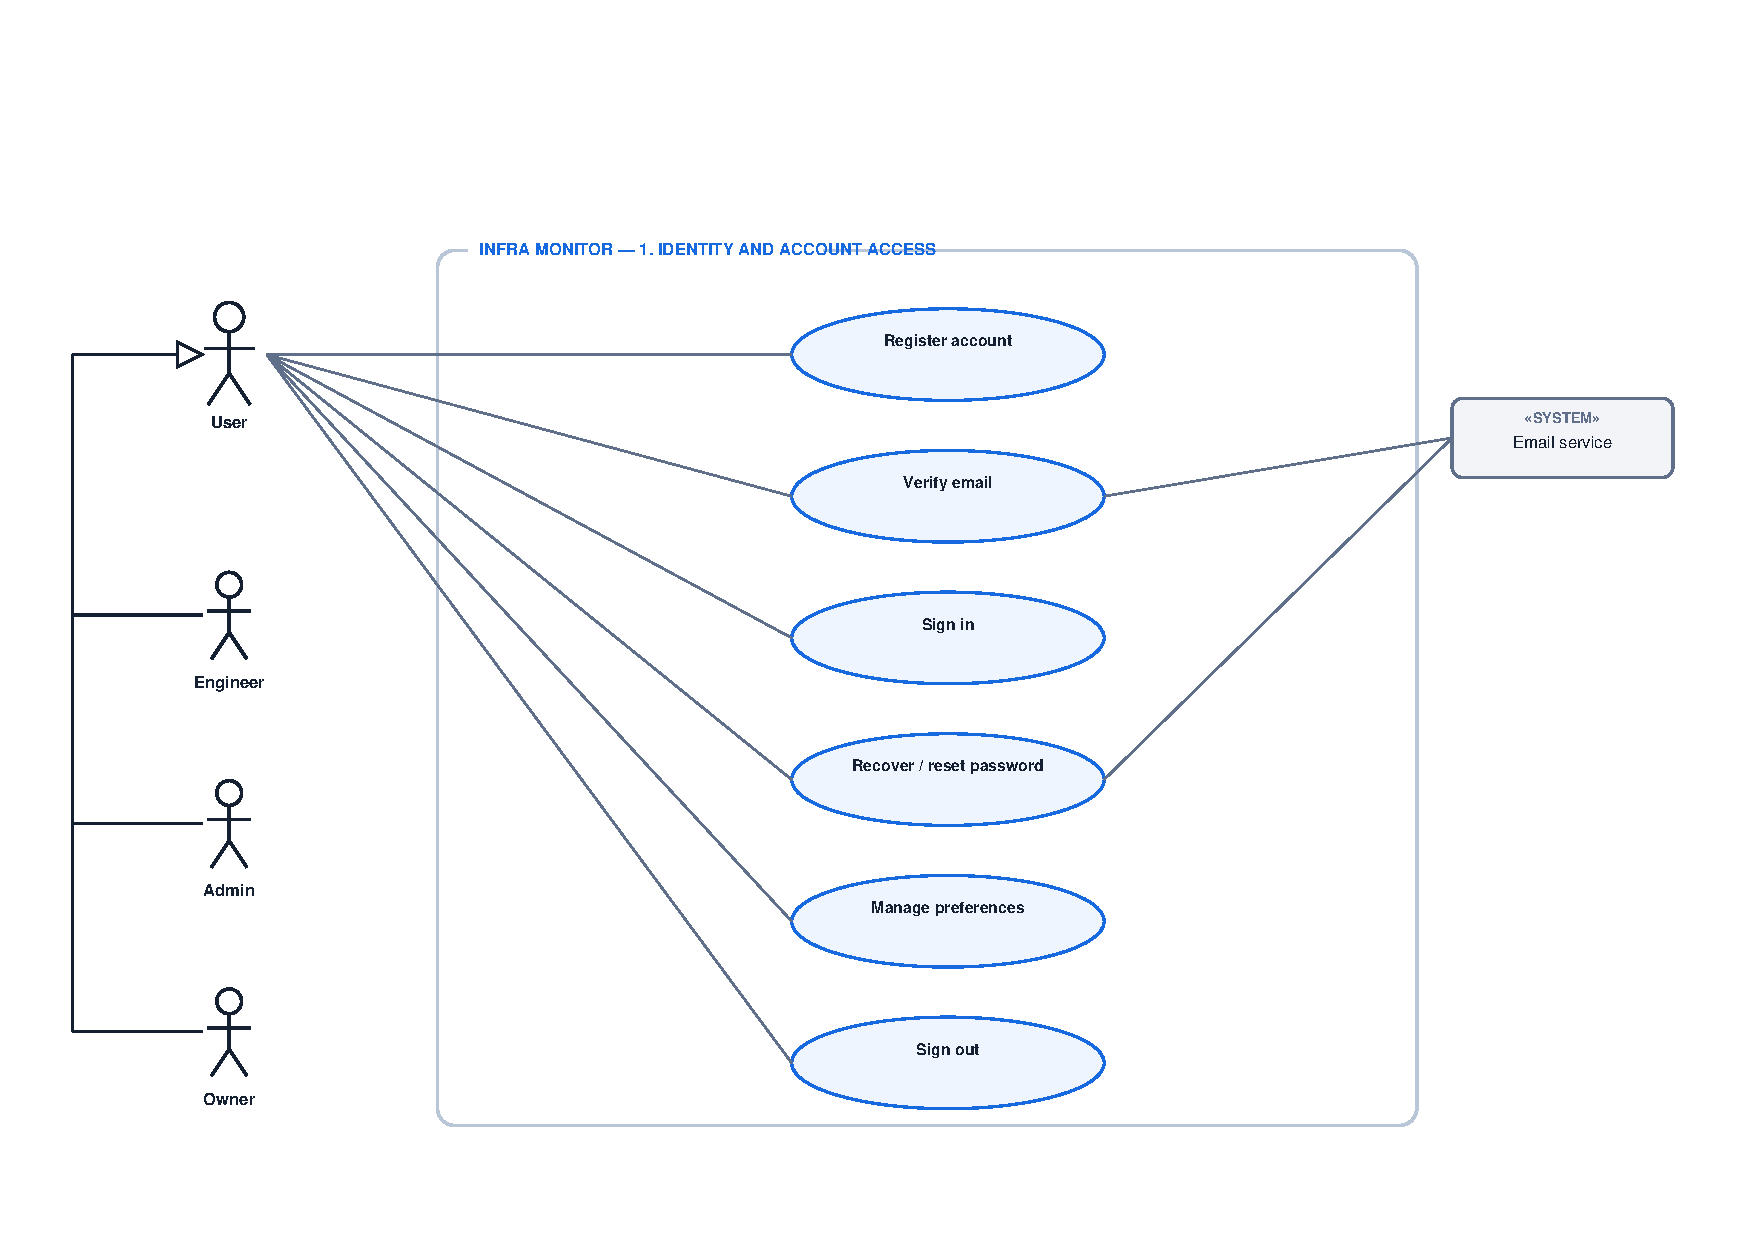
\includegraphics[width=0.95\textwidth]{infra_monitor_frontend_use_case_diagrams.pdf}
\caption{Use case diagram for Infra Monitor}\label{fig:usecase}
\end{figure}

The following subsections provide full textual specifications for each use case.

%-- UC-01 -------------------------------------------------------
\begin{table}[H]
\centering
\caption{Textual description of UC-01: User Account Registration}\label{tab:uc01}
\begin{tabularx}{\textwidth}{@{}l X@{}}
\toprule
\textbf{Use Case ID} & UC-01\\
\textbf{Name} & User Account Registration\\
\textbf{Actor(s)} & New User (unauthenticated)\\
\textbf{Precondition} & User has no existing account with the given email\\
\textbf{Postcondition} & Account created; email verified; user can log in\\
\textbf{Main flow} &
  1.~User submits \texttt{POST /api/auth/register/} with email, username, password.
  2.~System validates data via \texttt{RegisterView} (\texttt{accounts/views/}).
  3.~System creates \texttt{Users} record (\texttt{accounts/models/users.py}),
     generates a 6-digit OTP, stores it in \texttt{EmailVerificationOTP}, and
     sends it to the user's email.
  4.~User submits \texttt{POST /api/auth/verify-email/} with the OTP.
  5.~System marks \texttt{is\_email\_verified=True} and returns 200~OK.\\
\textbf{Alternative flow} &
  A1.~OTP expired: user calls \texttt{POST /api/auth/resend-otp/} to receive a fresh OTP.\\
\textbf{Exception flow} &
  E1.~Duplicate email: system returns HTTP~400 with field error.
  E2.~Invalid OTP: system returns HTTP~400 ``Invalid or expired OTP.''\\
\bottomrule
\end{tabularx}
\end{table}

%-- UC-02 -------------------------------------------------------
\begin{table}[H]
\centering
\caption{Textual description of UC-02: User Login}\label{tab:uc02}
\begin{tabularx}{\textwidth}{@{}l X@{}}
\toprule
\textbf{Use Case ID} & UC-02\\
\textbf{Name} & User Login\\
\textbf{Actor(s)} & Registered User\\
\textbf{Precondition} & Account exists; email verified\\
\textbf{Postcondition} & Access and refresh JWT tokens issued\\
\textbf{Main flow} &
  1.~User submits \texttt{POST /api/auth/login/} with email and password.
  2.~\texttt{LoginView} authenticates via Django auth; validates email is verified.
  3.~System issues JWT access token (short-lived) and refresh token (blacklistable).
  4.~Client stores tokens; subsequent requests include \texttt{Authorization: Bearer <access>}.\\
\textbf{Alternative flow} &
  A1.~Token expired: user calls \texttt{POST /api/auth/token/refresh/} with refresh token.\\
\textbf{Exception flow} &
  E1.~Wrong credentials: HTTP~401 ``Invalid credentials.''
  E2.~Email not verified: HTTP~403 ``Email not verified.''\\
\bottomrule
\end{tabularx}
\end{table}

%-- UC-03 -------------------------------------------------------
\begin{table}[H]
\centering
\caption{Textual description of UC-03: Organisation Creation \& Member Joining}\label{tab:uc03}
\begin{tabularx}{\textwidth}{@{}l X@{}}
\toprule
\textbf{Use Case ID} & UC-03\\
\textbf{Name} & Organisation Creation \& Member Joining\\
\textbf{Actor(s)} & Authenticated User (becomes Owner); other Users (Engineers)\\
\textbf{Precondition} & All users authenticated and email-verified\\
\textbf{Postcondition} & Organisation exists; Owner membership created; Engineers pending approval\\
\textbf{Main flow} &
  1.~User calls \texttt{POST /api/organizations/} with name and summary.
  2.~System creates \texttt{Organisation} and a \texttt{VictoriaMetricsTenant}, assigns
     the caller as OWNER with \texttt{approved=True}.
  3.~Other users call \texttt{POST /api/organizations/<id>/members/} to request membership
     (default role ENGINEER, \texttt{approved=False}).
  4.~Owner calls \texttt{PATCH /api/organizations/<id>/members/<uid>/} to approve.\\
\textbf{Alternative flow} &
  A1.~Owner invites Admin: sets role ADMIN and approved=True immediately.\\
\textbf{Exception flow} &
  E1.~Duplicate membership: HTTP~400 unique constraint violation.
  E2.~Non-Owner tries to approve: HTTP~403 ``Only the owner may approve memberships.''\\
\bottomrule
\end{tabularx}
\end{table}

%-- UC-04 -------------------------------------------------------
\begin{table}[H]
\centering
\caption{Textual description of UC-04: Server Setup \& Metric Collection}\label{tab:uc04}
\begin{tabularx}{\textwidth}{@{}l X@{}}
\toprule
\textbf{Use Case ID} & UC-04\\
\textbf{Name} & Server Setup \& Metric Collection\\
\textbf{Actor(s)} & Organisation Owner / Admin\\
\textbf{Precondition} & Organisation exists; user has Owner or Admin role\\
\textbf{Postcondition} & Server record created; Alloy agent installed on host; telemetry flowing\\
\textbf{Main flow} &
  1.~Admin calls \texttt{POST /api/organizations/<oid>/servers/} with name, hostname, environment.
  2.~System creates \texttt{Servers} record (\texttt{servers/models/servers.py}) and an
     \texttt{EnrollmentToken}.
  3.~Admin downloads the generated Alloy installer script from
     \texttt{GET /api/monitoring/installer/}.
  4.~Admin runs script on the target Linux host; Alloy agent calls back to
     \texttt{POST /api/monitoring/enroll/} with the token, registering the host.
  5.~Alloy writes Prometheus remote-write metrics to
     \texttt{POST /api/metrics/write}, which proxies to VictoriaMetrics vminsert.
  6.~Dashboard reads metrics via \texttt{GET /api/organizations/<oid>/servers/<sid>/metrics/}.\\
\textbf{Alternative flow} &
  A1.~Token expired: Admin regenerates token from \texttt{POST /api/monitoring/enroll/token/}.\\
\textbf{Exception flow} &
  E1.~Duplicate hostname in org: HTTP~400.
  E2.~VictoriaMetrics unreachable: vminsert health-check fails; Compose restart policy applies.\\
\bottomrule
\end{tabularx}
\end{table}

%-- UC-05 -------------------------------------------------------
\begin{table}[H]
\centering
\caption{Textual description of UC-05: Incident \& Anomaly Assignment}\label{tab:uc05}
\begin{tabularx}{\textwidth}{@{}l X@{}}
\toprule
\textbf{Use Case ID} & UC-05\\
\textbf{Name} & Incident and Anomaly Assignment\\
\textbf{Actor(s)} & Organisation Admin (assigns); Engineer (acknowledges/resolves)\\
\textbf{Precondition} & Incident or anomaly record exists in system; Engineer membership approved\\
\textbf{Postcondition} & Incident/anomaly has assigned Engineer; lifecycle progresses\\
\textbf{Main flow} &
  1.~Admin calls \texttt{PATCH /api/organizations/<oid>/incidents/<iid>/} with
     \texttt{assigned\_to} UUID of an approved Engineer.
  2.~System validates via \texttt{Incident.clean()} that the assignee is an approved
     Engineer in the organisation (\texttt{incident/models/incident.py}).
  3.~Engineer receives Firebase push notification (\texttt{notifications/}).
  4.~Engineer updates status to INVESTIGATING, then RESOLVED with resolution notes.\\
\textbf{Alternative flow} &
  A1.~Engineer is re-assigned: previous assignment is overwritten; event logged.\\
\textbf{Exception flow} &
  E1.~Assignee not an Engineer: HTTP~400 validation error from \texttt{Incident.clean()}.\\
\bottomrule
\end{tabularx}
\end{table}

%-- UC-06 -------------------------------------------------------
\begin{table}[H]
\centering
\caption{Textual description of UC-06: AI Chatbot Conversation}\label{tab:uc06}
\begin{tabularx}{\textwidth}{@{}l X@{}}
\toprule
\textbf{Use Case ID} & UC-06\\
\textbf{Name} & AI Chatbot Conversation (Anomaly Advisory)\\
\textbf{Actor(s)} & Authenticated Organisation Member\\
\textbf{Precondition} & At least one anomaly detection exists in the organisation\\
\textbf{Postcondition} & Conversation and messages persisted; Gemini response delivered\\
\textbf{Main flow} &
  1.~User calls \texttt{POST /api/organizations/<oid>/assistant/conversations/} with
     \texttt{anomaly\_id}.
  2.~System creates or retrieves \texttt{AssistantConversation}
     (\texttt{ai/models/assistant\_conversation.py}).
  3.~User calls \texttt{POST /api/organizations/<oid>/assistant/ws-ticket/} to get a
     one-use WebSocket ticket (SHA-256 hashed, 60s TTL via
     \texttt{ai/services.py:issue\_websocket\_ticket}).
  4.~User connects to WebSocket \texttt{/ws/organizations/<oid>/assistant/conversations/<cid>/}.
  5.~System authenticates ticket (\texttt{consume\_websocket\_ticket}), loads anomaly
     evidence snapshot, and streams Gemini response to the client.
  6.~System persists user message and AI response as \texttt{AssistantMessage} records.\\
\textbf{Alternative flow} &
  A1.~Gemini not configured (\texttt{GEMINI\_API\_KEY} absent): error ``gemini\_not\_configured''.\\
\textbf{Exception flow} &
  E1.~Ticket expired or already used: WebSocket closed with error code.\\
\bottomrule
\end{tabularx}
\end{table}

%-- UC-07 -------------------------------------------------------
\begin{table}[H]
\centering
\caption{Textual description of UC-07: Request Shield Monitoring}\label{tab:uc07}
\begin{tabularx}{\textwidth}{@{}l X@{}}
\toprule
\textbf{Use Case ID} & UC-07\\
\textbf{Name} & Request Shield -- HTTP Traffic Classification\\
\textbf{Actor(s)} & Organisation Admin (review); Automated System (classify)\\
\textbf{Precondition} & Server enrolled; Alloy agent forwarding access logs; Shield enabled\\
\textbf{Postcondition} & Requests classified GREEN/GRAY/RED; threat suggestions generated for suspicious IPs\\
\textbf{Main flow} &
  1.~Alloy agent submits batches of access log lines to
     \texttt{POST /api/internal/request-logs/ingest/}.
  2.~\texttt{sanitize/middleware.py} also captures PLATFORM-source requests.
  3.~Celery beat task (\texttt{sanitize/tasks.py}) sends unclassified batches to
     ML service \texttt{POST /classify/} every 30~s.
  4.~ML service returns zone (GREEN/GRAY/RED) and confidence per request.
  5.~System escalates GRAY requests to Gemini for deeper analysis when configured.
  6.~When an IP exceeds threshold, system generates a \texttt{ThreatSuggestion}.
  7.~Admin reviews via \texttt{GET /api/organizations/<oid>/request-shield/analytics/}
     and acts on suggestions via \texttt{POST .../suggestions/<id>/action/}.\\
\textbf{Alternative flow} &
  A1.~ML service unavailable: requests remain UNCLASSIFIED; retried on next task run.\\
\textbf{Exception flow} &
  E1.~Batch exceeds 500 requests: HTTP~400 from ML service schema validation.\\
\bottomrule
\end{tabularx}
\end{table}

%-- UC-08 -------------------------------------------------------
\begin{table}[H]
\centering
\caption{Textual description of UC-08: Password Reset}\label{tab:uc08}
\begin{tabularx}{\textwidth}{@{}l X@{}}
\toprule
\textbf{Use Case ID} & UC-08\\
\textbf{Name} & Password Reset via OTP\\
\textbf{Actor(s)} & Registered User (unauthenticated)\\
\textbf{Precondition} & User has an existing account\\
\textbf{Postcondition} & User's password updated; old sessions invalidated\\
\textbf{Main flow} &
  1.~User calls \texttt{POST /api/auth/forgot-password/} with email.
  2.~System creates \texttt{PasswordResetOTP} and emails it.
  3.~User calls \texttt{POST /api/auth/reset-password/} with email, OTP, new password.
  4.~System validates OTP, updates password, marks OTP used.\\
\textbf{Exception flow} &
  E1.~OTP expired or already used: HTTP~400.\\
\bottomrule
\end{tabularx}
\end{table}

\section{Activity Diagram}

Activity diagrams illustrate the workflow of major processes.
\Cref{fig:act_login} shows the account login flow; \Cref{fig:act_server} shows
server setup and metric collection; \Cref{fig:act_incident} shows incident and
anomaly assignment; \Cref{fig:act_chatbot} shows the chatbot conversation flow;
\Cref{fig:act_shield} shows the Request Shield classification flow.

\begin{figure}[H]
\centering
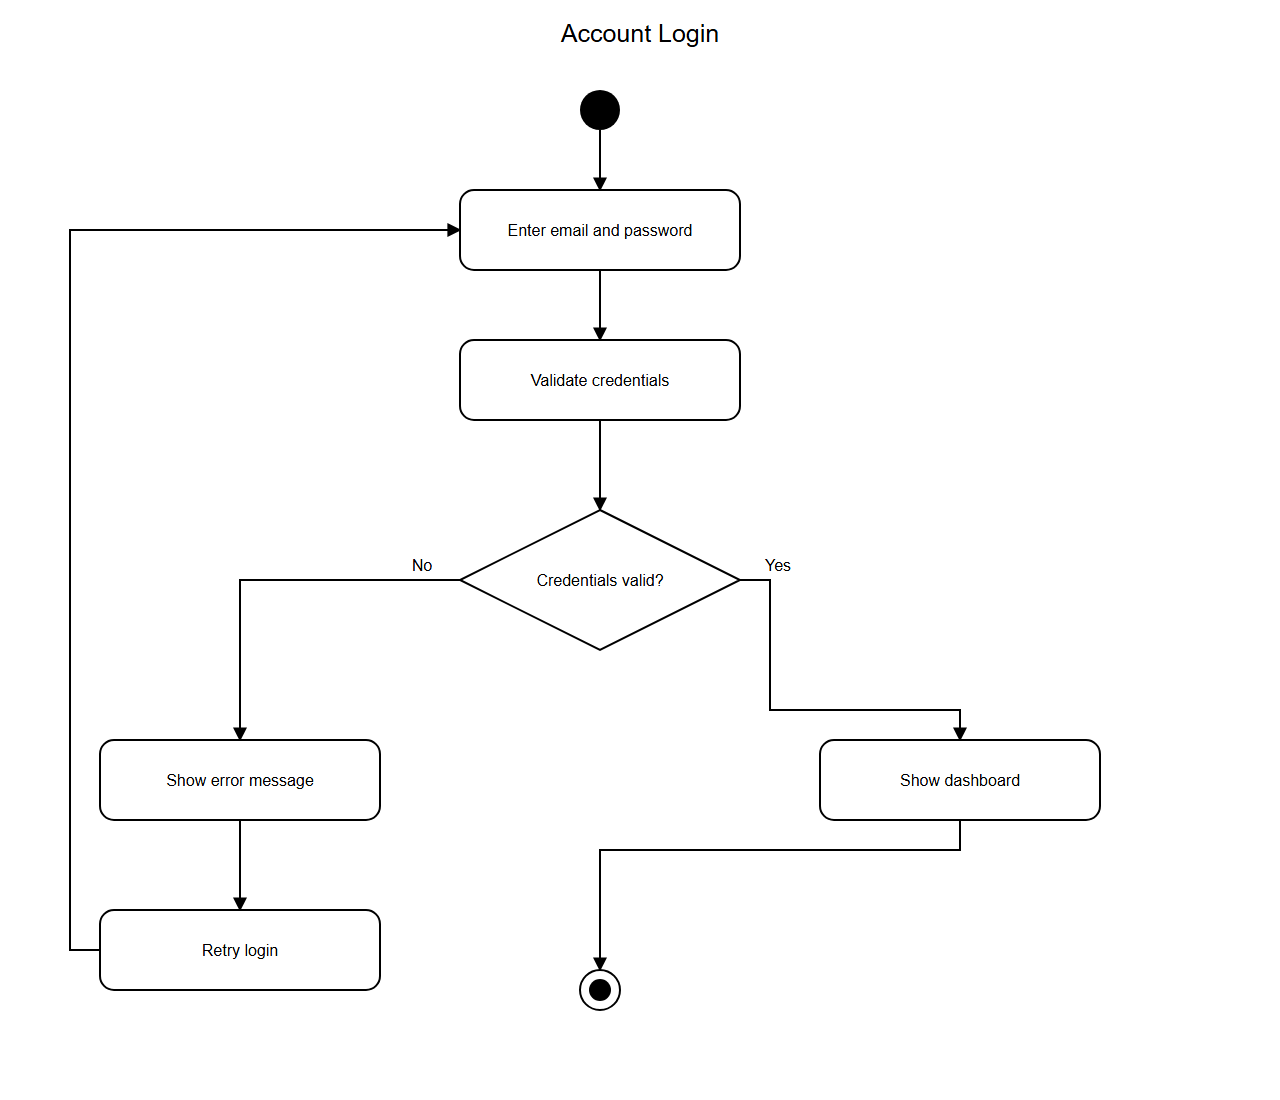
\includegraphics[width=0.78\textwidth]{Account_Login_Activity_Diagram.png}
\caption{Activity diagram: Account Login}\label{fig:act_login}
\end{figure}

\begin{figure}[H]
\centering
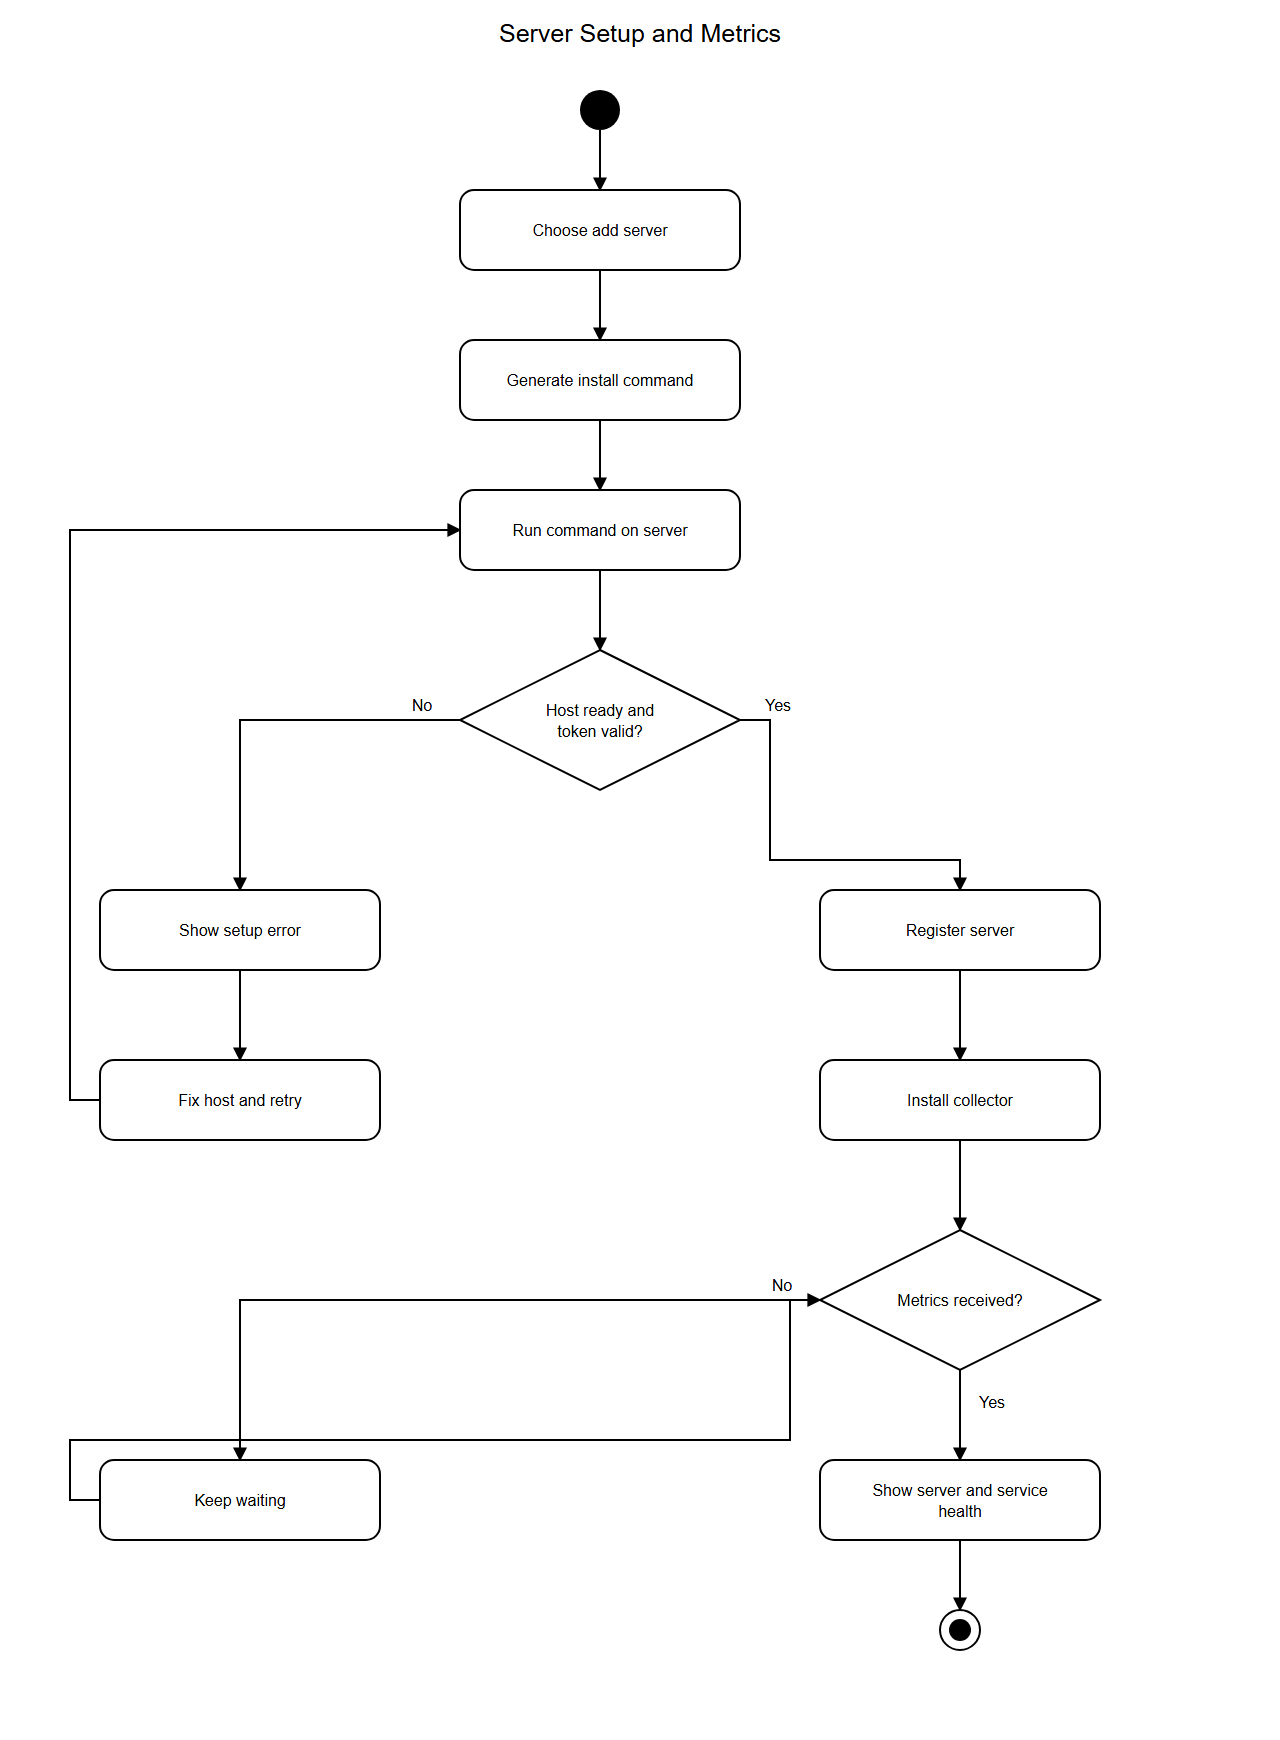
\includegraphics[width=0.78\textwidth]{Server_Setup_and_Metrics_Activity_Diagram.png}
\caption{Activity diagram: Server Setup and Metric Collection}\label{fig:act_server}
\end{figure}

\begin{figure}[H]
\centering
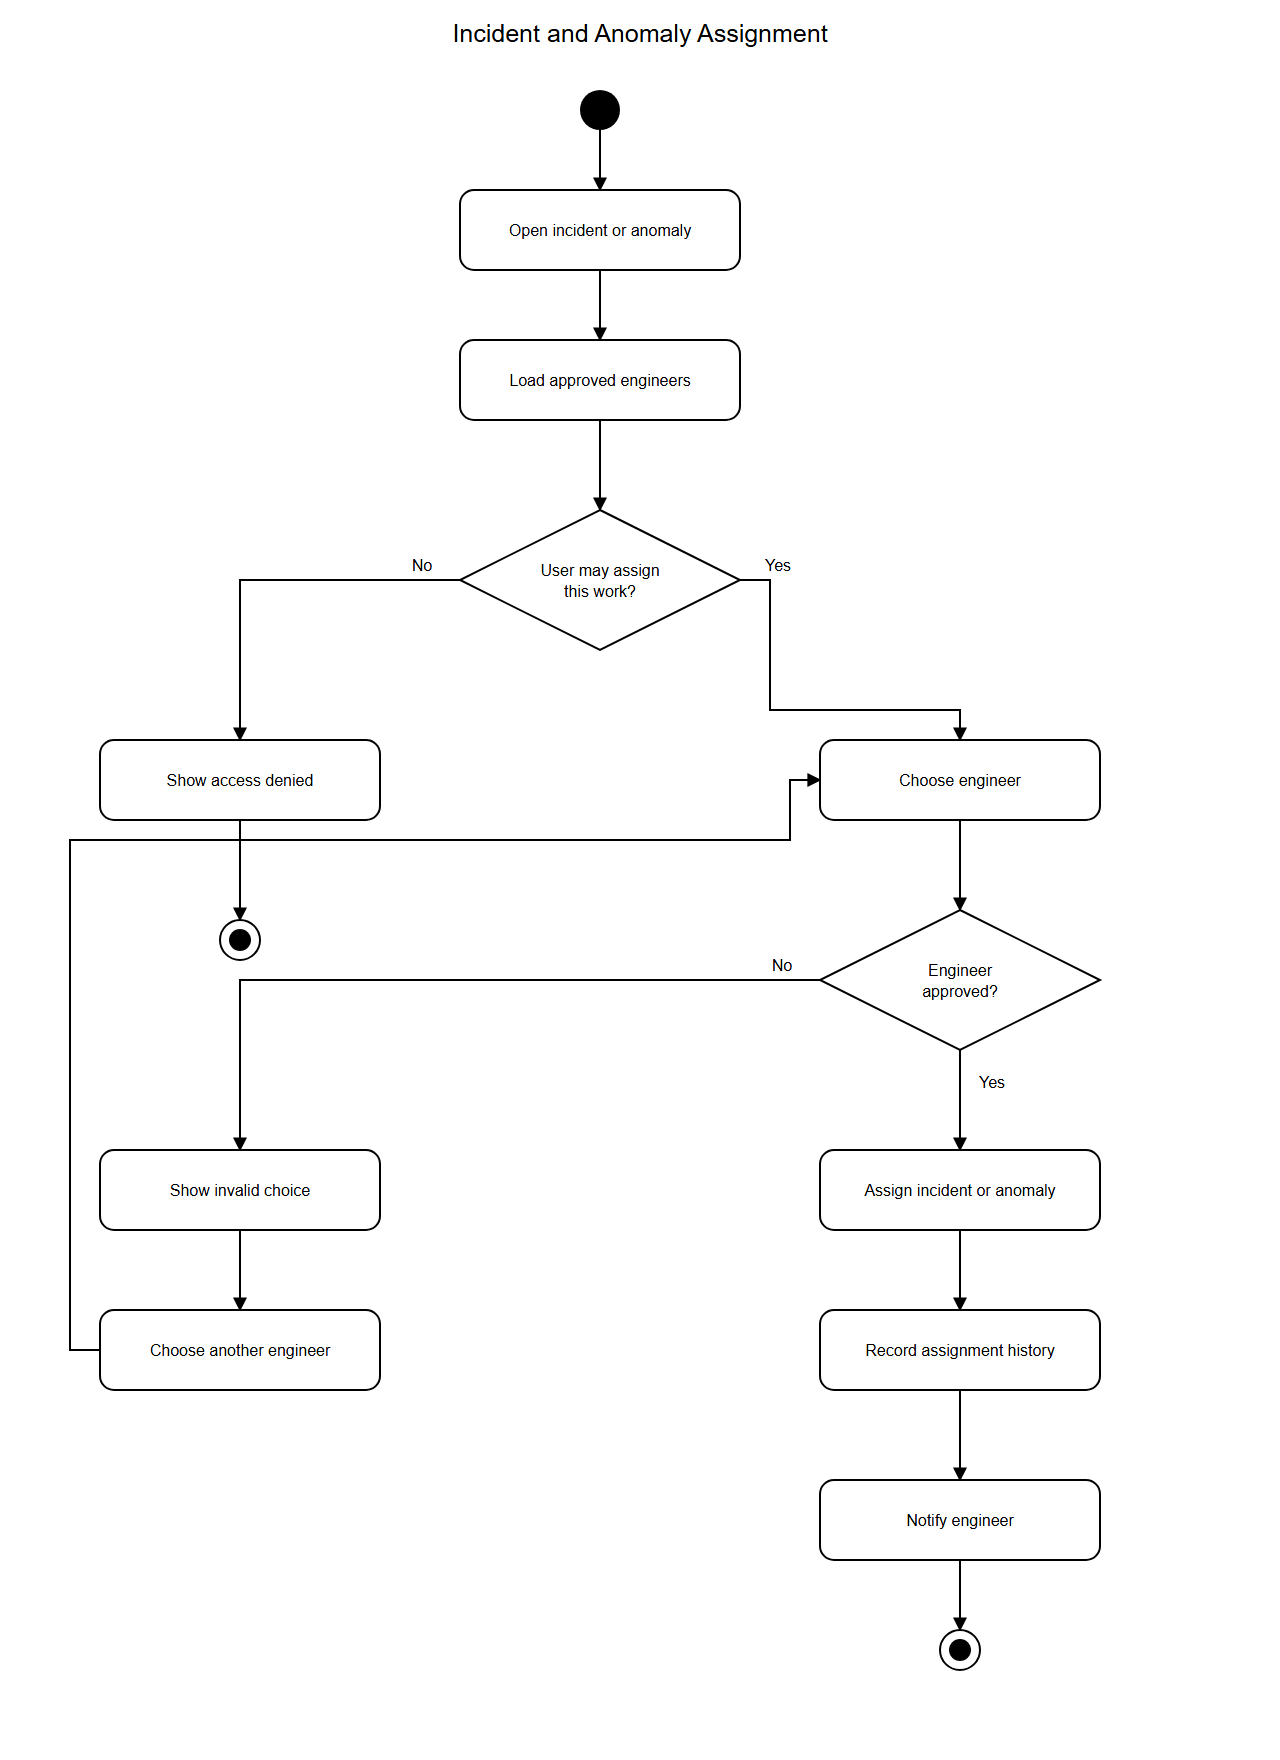
\includegraphics[width=0.78\textwidth]{Incident_and_Anomaly_Assignment_Activity_Diagram.png}
\caption{Activity diagram: Incident and Anomaly Assignment}\label{fig:act_incident}
\end{figure}

\begin{figure}[H]
\centering
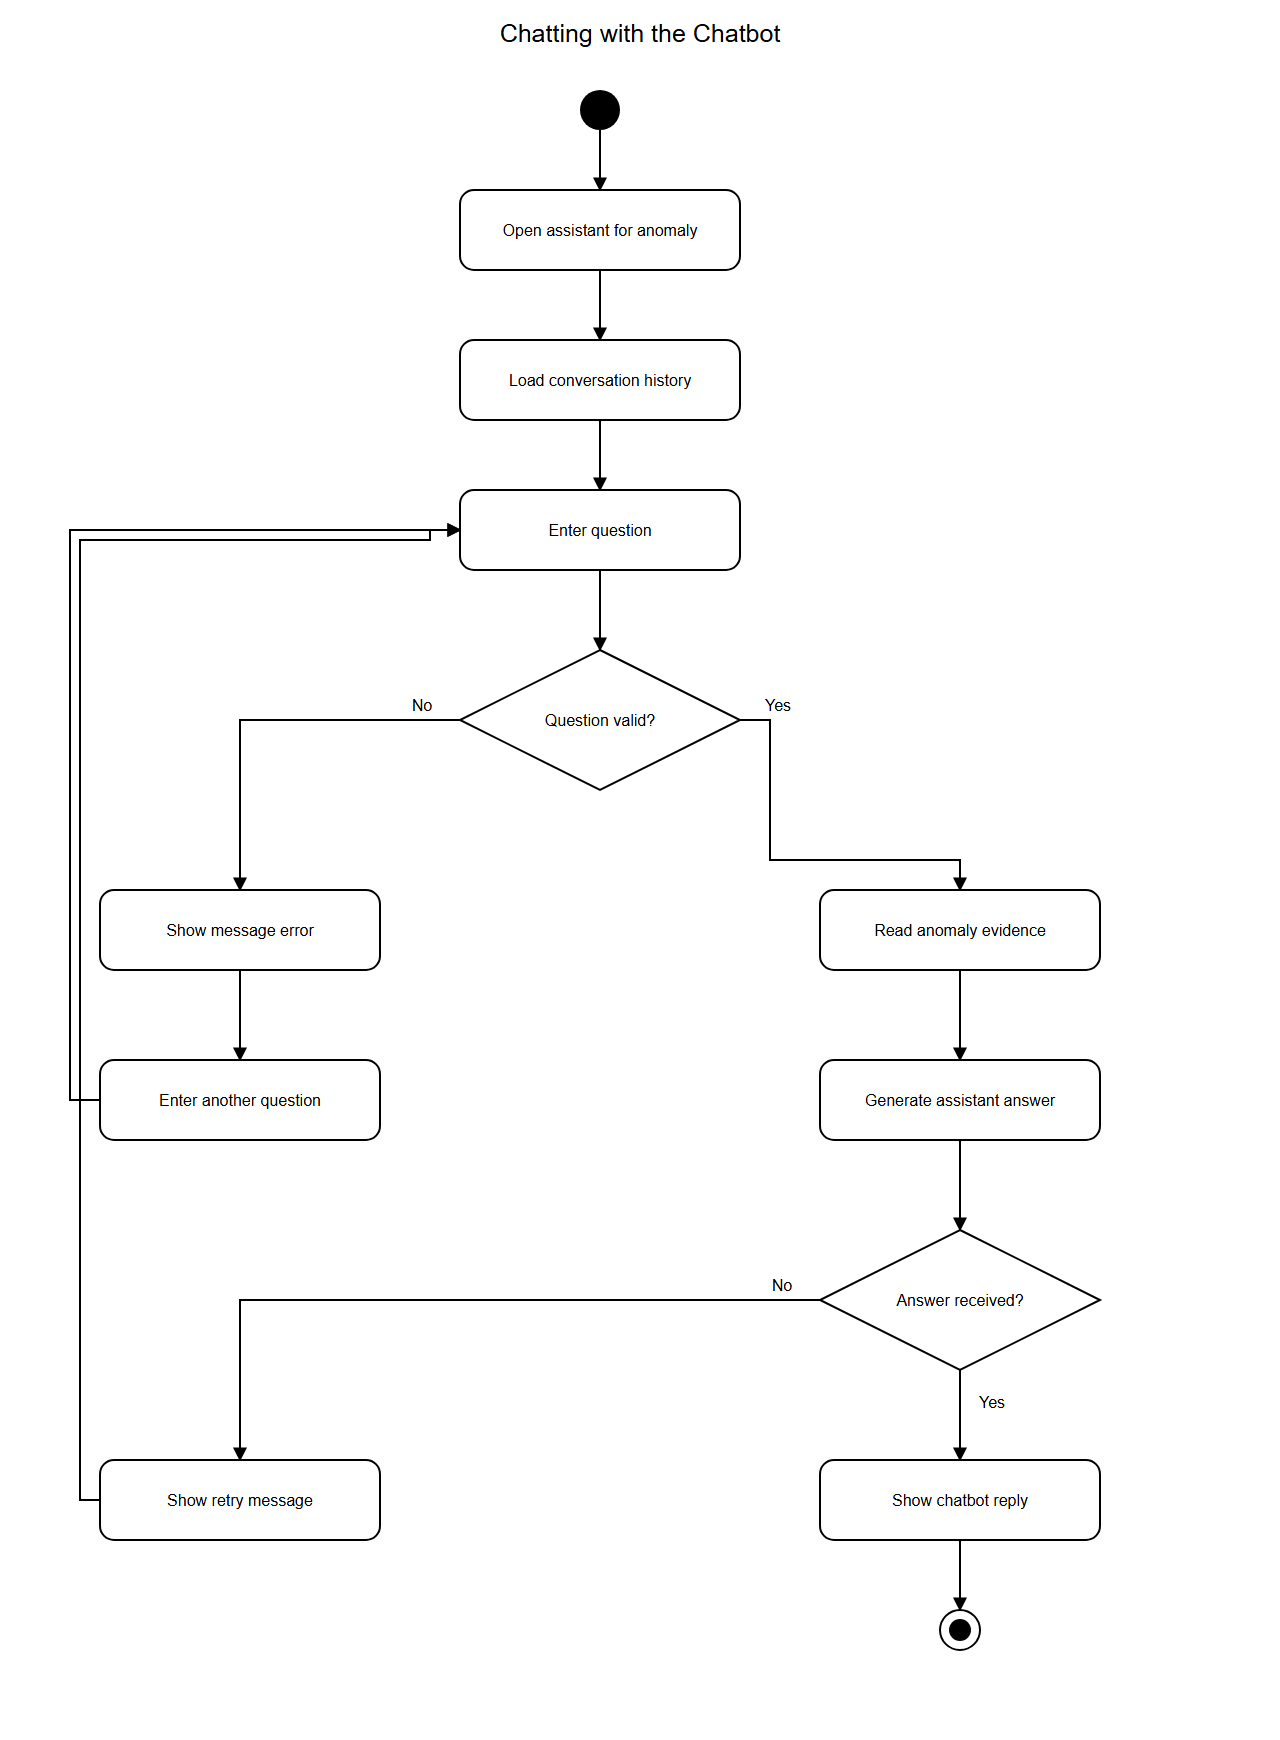
\includegraphics[width=0.78\textwidth]{Chatbot_Conversation_Activity_Diagram.png}
\caption{Activity diagram: AI Chatbot Conversation}\label{fig:act_chatbot}
\end{figure}

\begin{figure}[H]
\centering
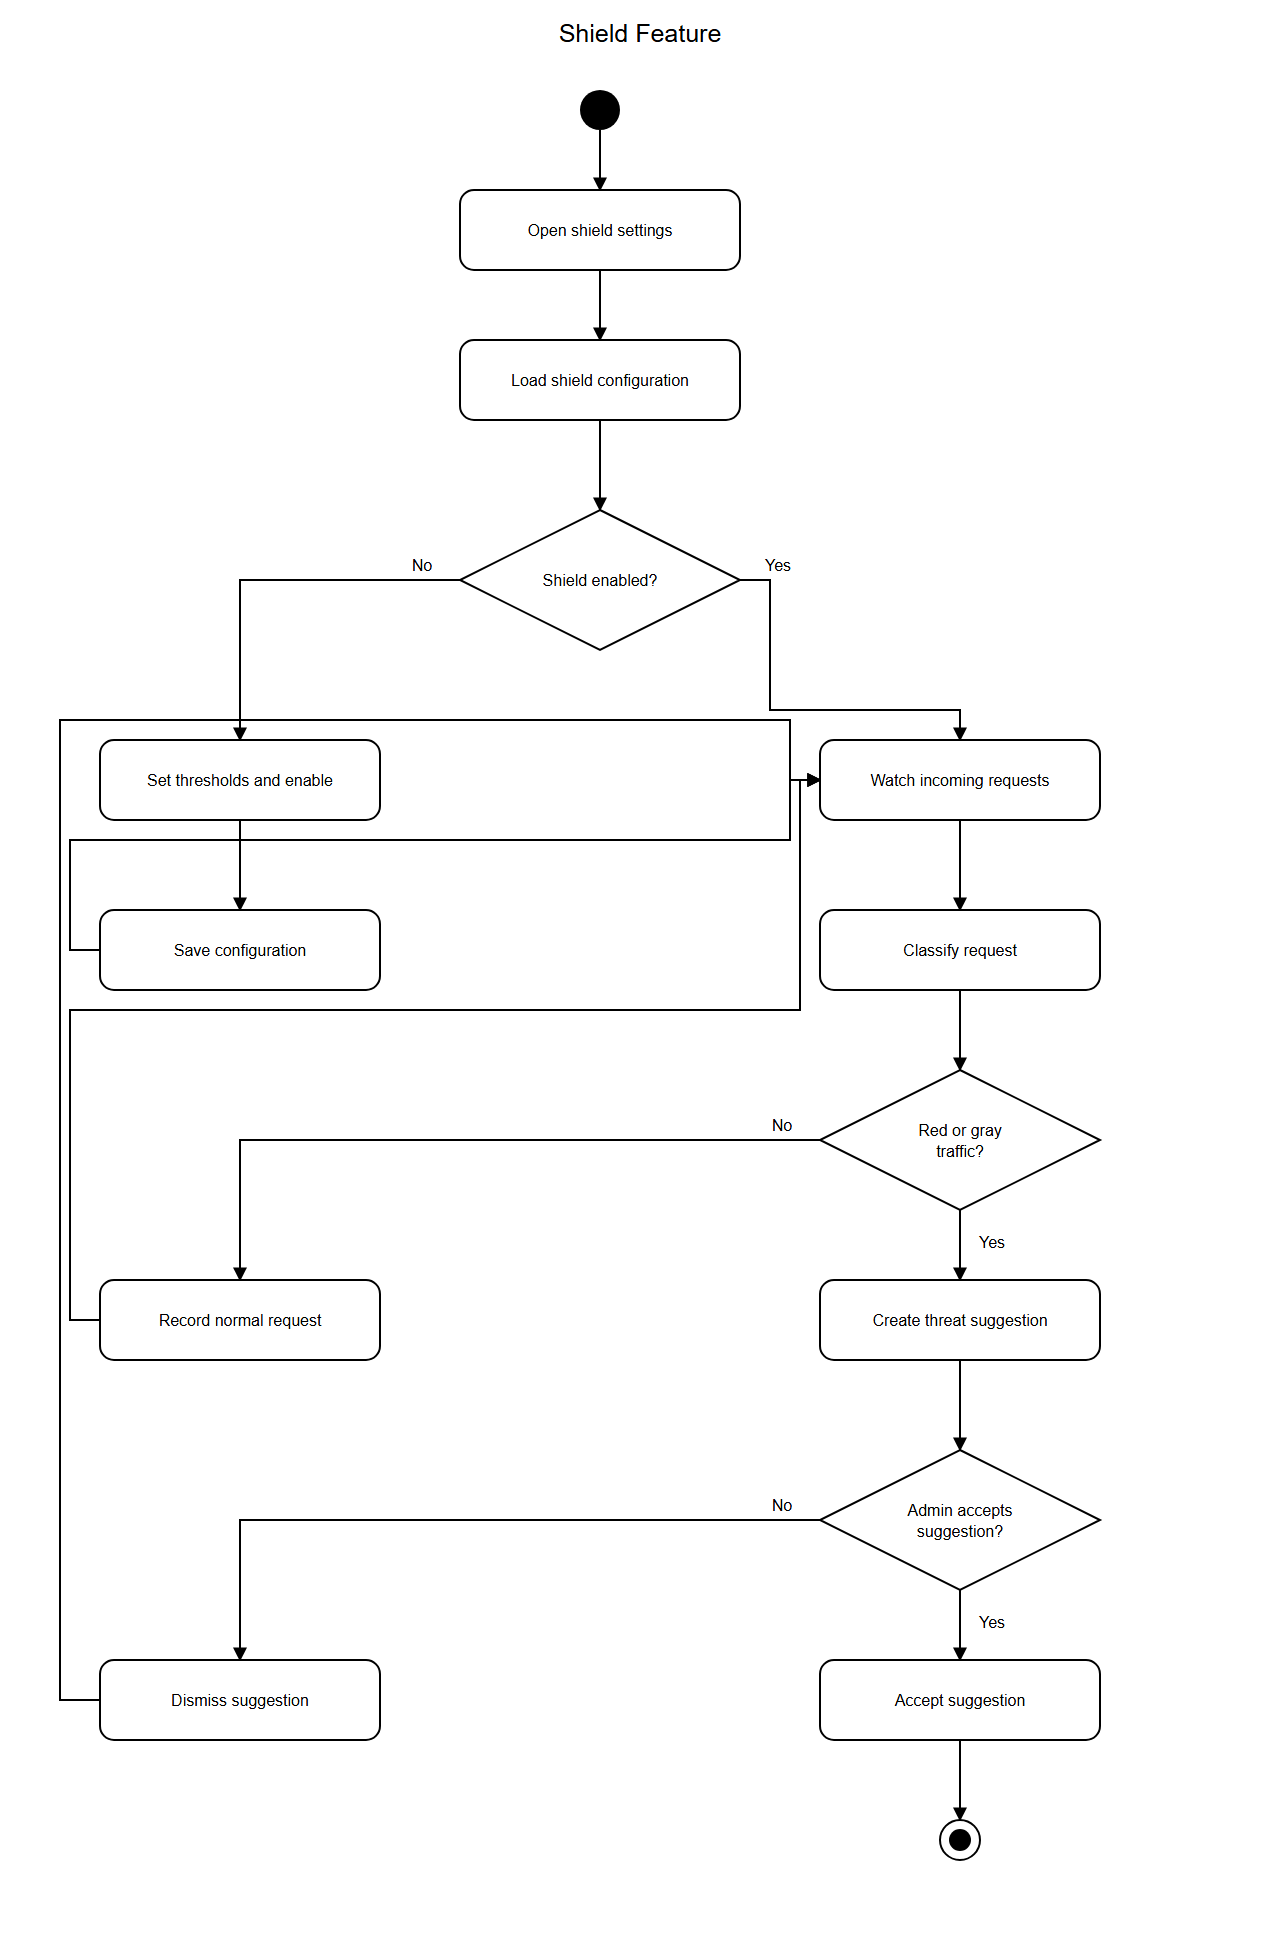
\includegraphics[width=0.78\textwidth]{Shield_Feature_Activity_Diagram.png}
\caption{Activity diagram: Request Shield Feature}\label{fig:act_shield}
\end{figure}

\begin{figure}[H]
\centering
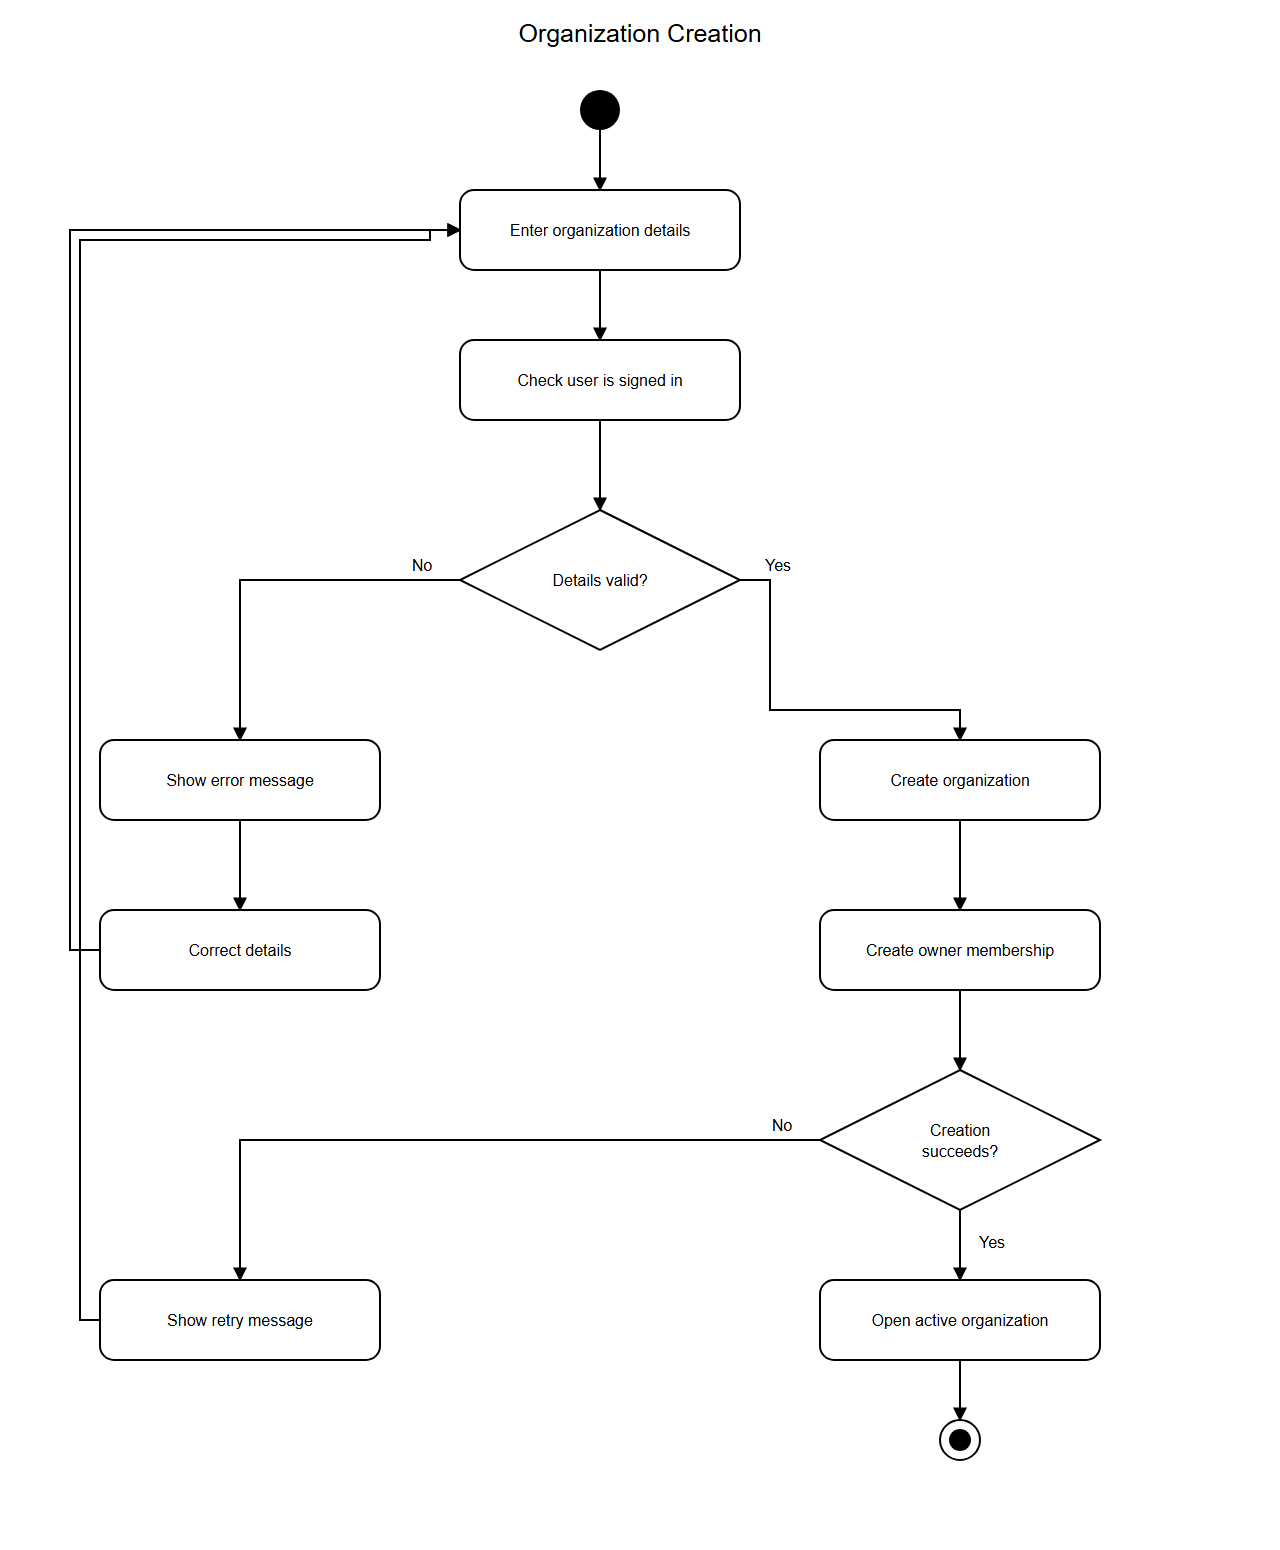
\includegraphics[width=0.78\textwidth]{Organization_Creation_Activity_Diagram.png}
\caption{Activity diagram: Organisation Creation}\label{fig:act_org}
\end{figure}

\begin{figure}[H]
\centering
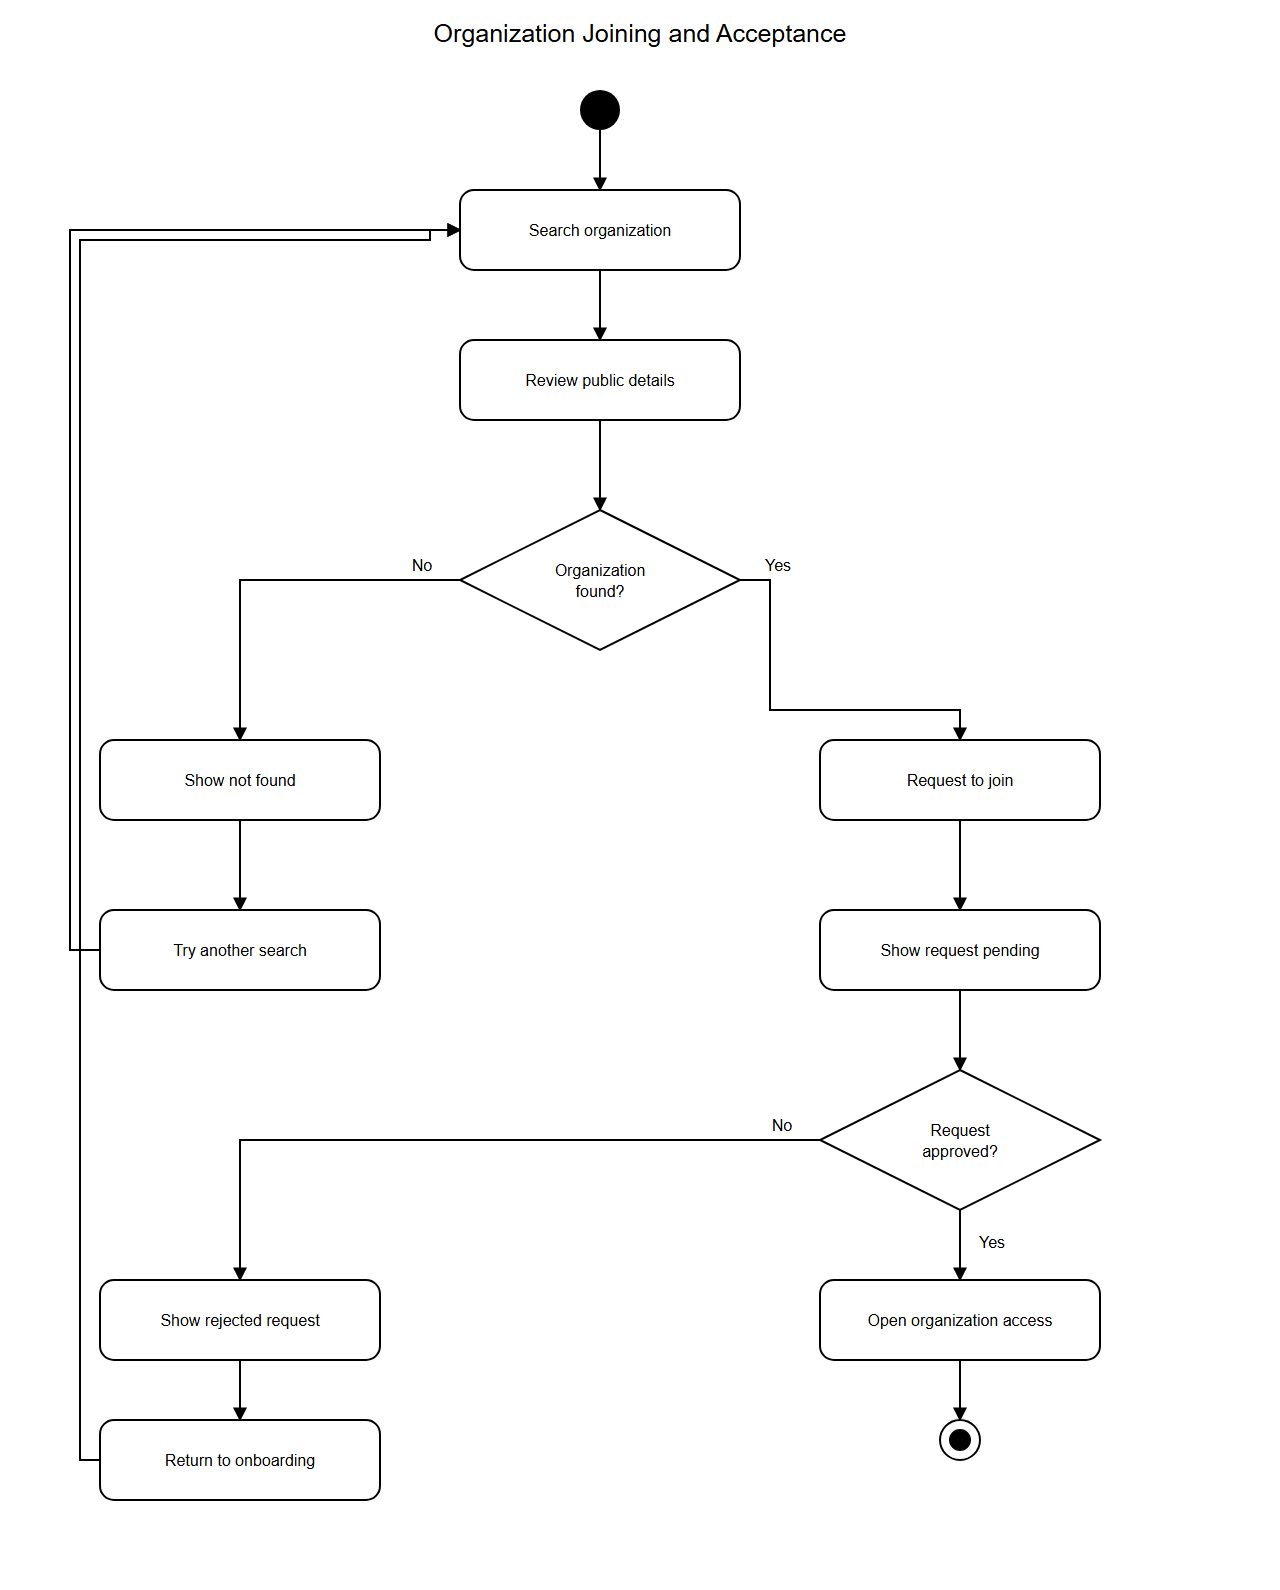
\includegraphics[width=0.78\textwidth]{Organization_Joining_and_Acceptance_Activity_Diagram.png}
\caption{Activity diagram: Organisation Joining and Acceptance}\label{fig:act_join}
\end{figure}

\section{Static Model -- Class Diagram}

The class diagram (\Cref{fig:class}) depicts the core domain entities of Infra
Monitor as Django models, their attributes, and relationships.  Key entities
include \texttt{Users}, \texttt{Organization}, \texttt{OrganizationMembership},
\texttt{Servers}, \texttt{Service}, \texttt{AnomalyDetection}, \texttt{Alert},
\texttt{Incident}, \texttt{AssistantConversation}, \texttt{RequestLog}, and
\texttt{ThreatSuggestion}.  Many-to-many relationships (e.g., service admin
assignments) are resolved through explicit junction models
(\texttt{ServiceAdminAssignment}).

\begin{figure}[H]
\centering
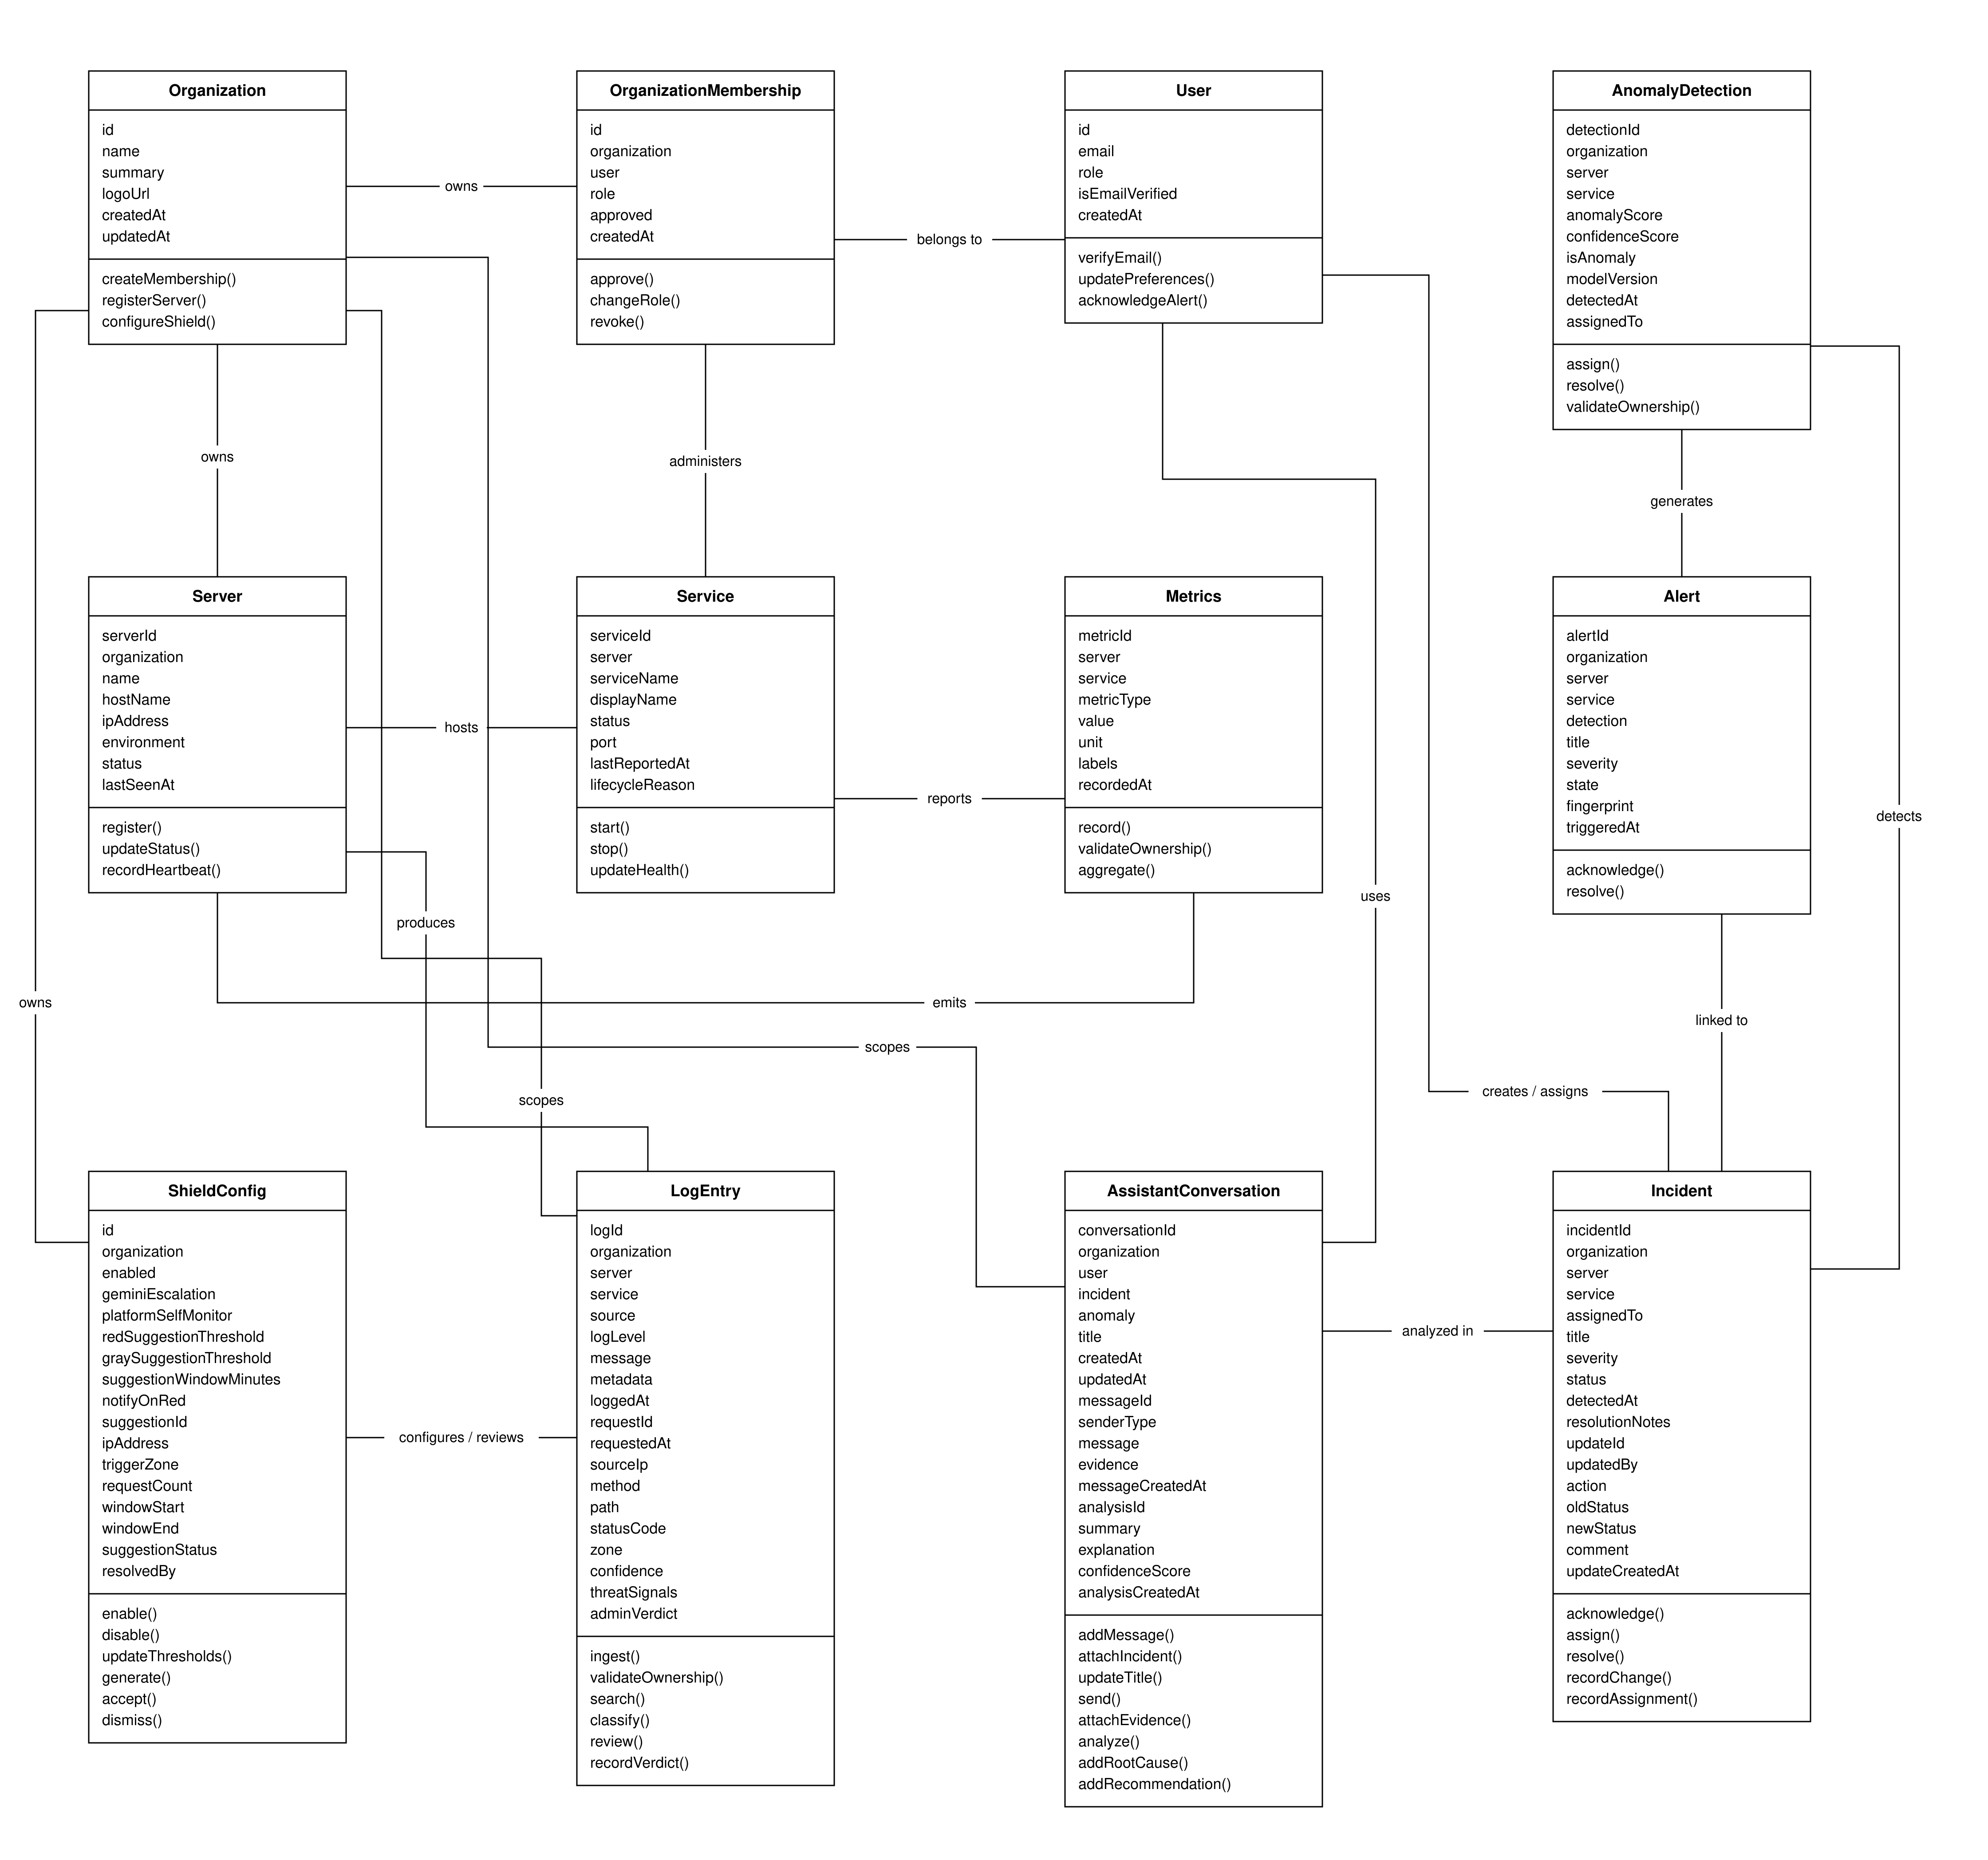
\includegraphics[width=0.98\textwidth]{class_diagram.png}
\caption{Class diagram for Infra Monitor domain model}\label{fig:class}
\end{figure}

\section{Dynamic Model -- Sequence Diagram}

Sequence diagrams illustrate object interactions for the key scenarios.

\begin{figure}[H]
\centering
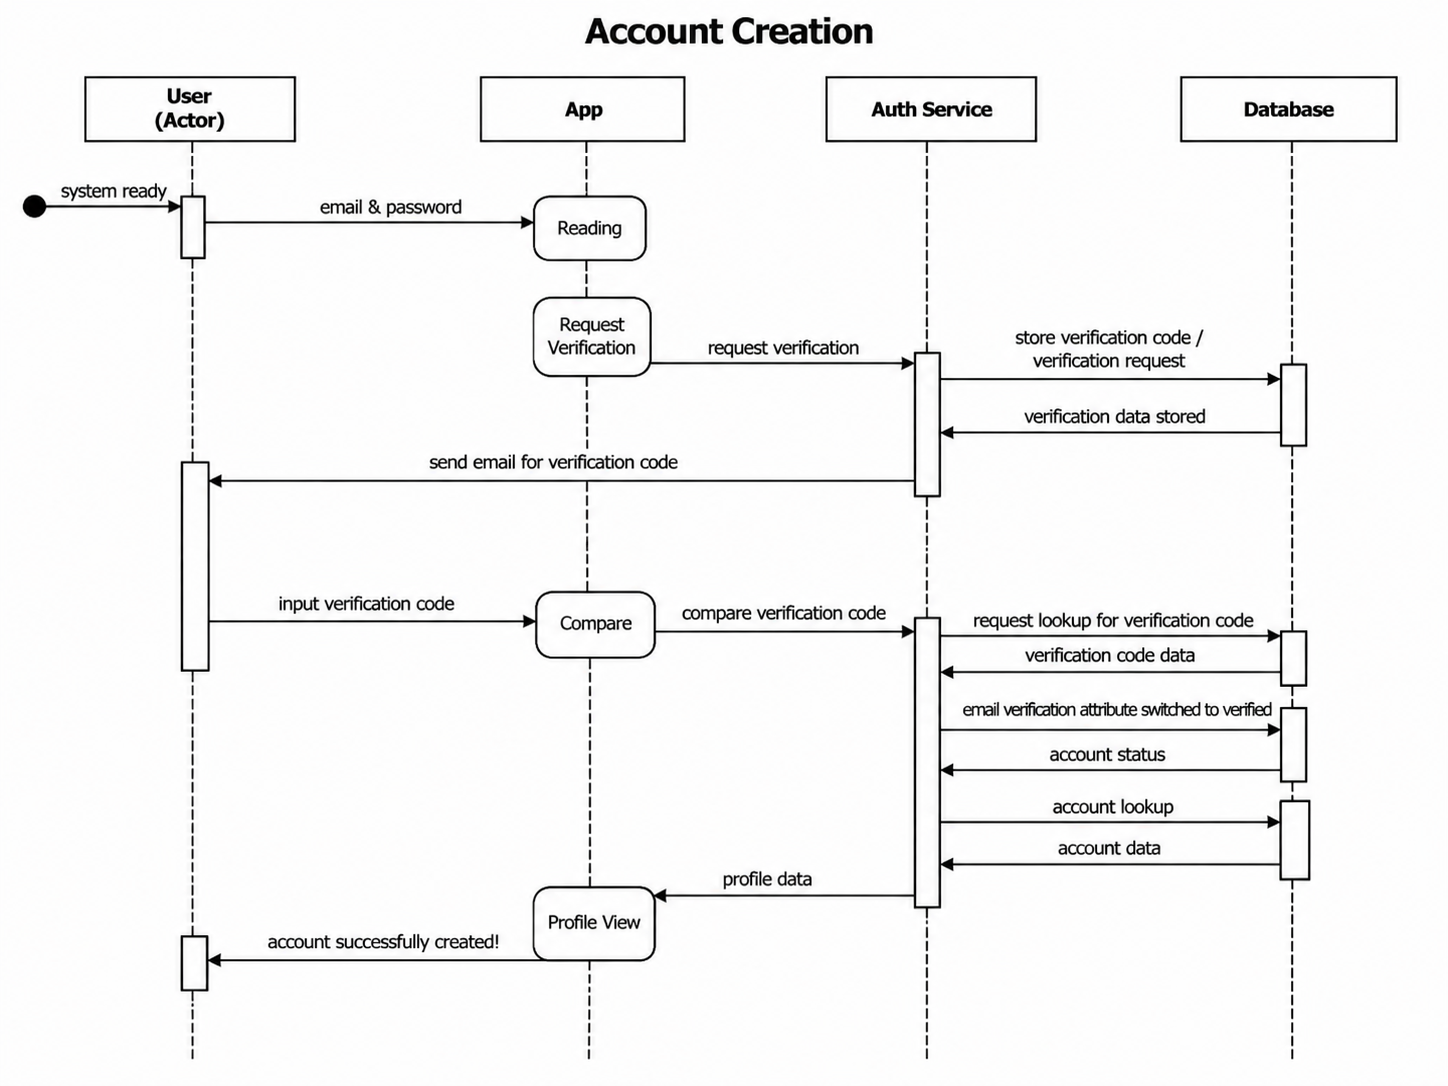
\includegraphics[width=0.92\textwidth]{Account_Creation_Sequence_Diagram__2_.png}
\caption{Sequence diagram: Account Registration and Email Verification}\label{fig:seq_reg}
\end{figure}

\begin{figure}[H]
\centering
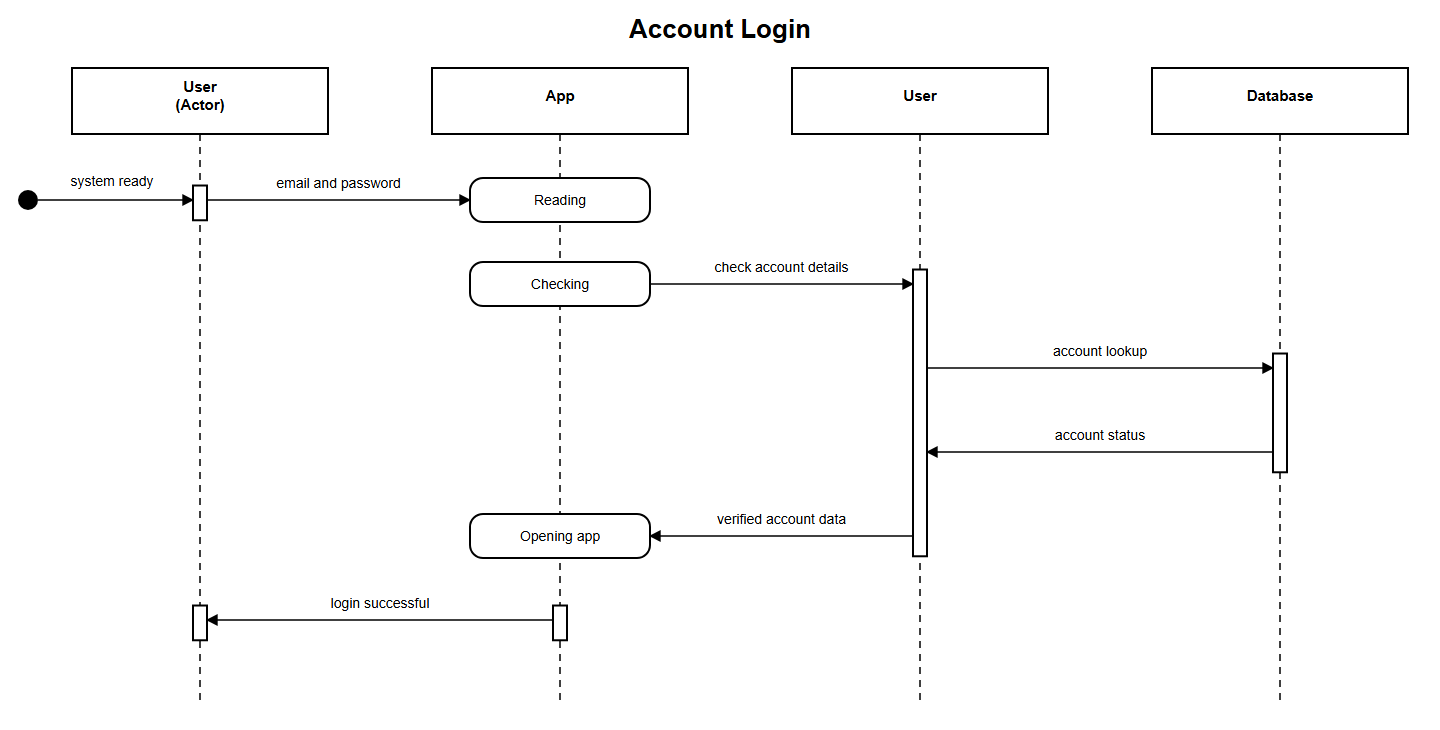
\includegraphics[width=0.92\textwidth]{Account_Login_Sequence_Diagram_1_.png}
\caption{Sequence diagram: User Login and JWT Issuance}\label{fig:seq_login}
\end{figure}

\begin{figure}[H]
\centering
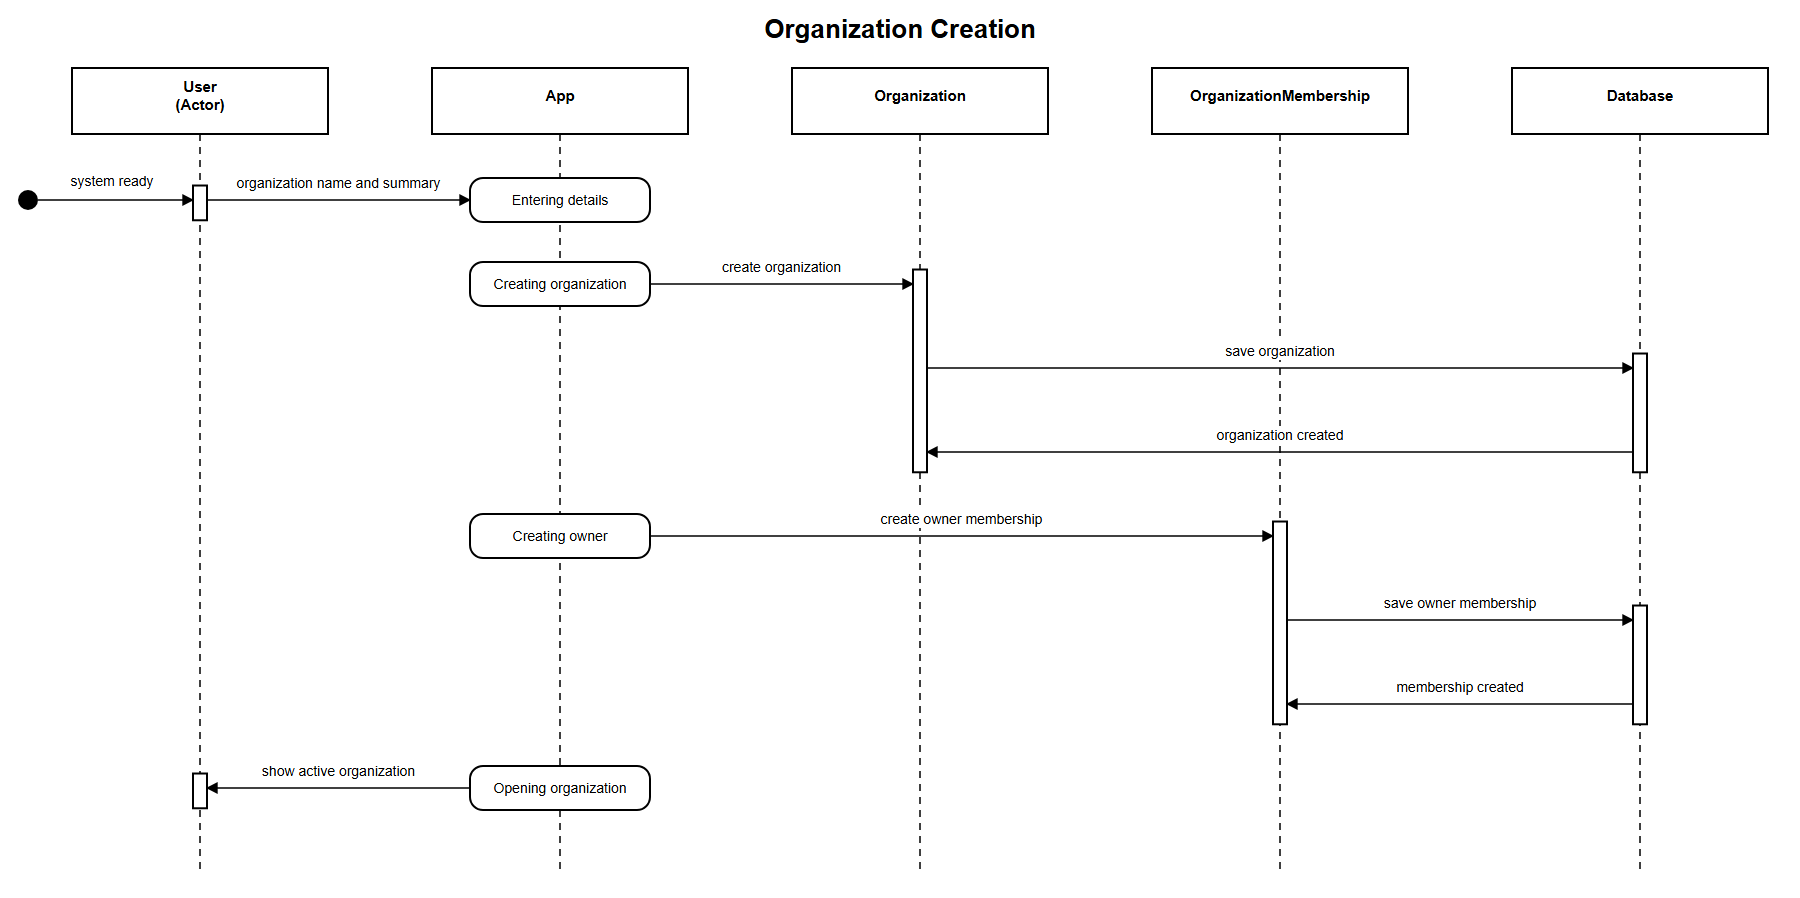
\includegraphics[width=0.92\textwidth]{Organization_Creation_Sequence_Diagram.png}
\caption{Sequence diagram: Organisation Creation}\label{fig:seq_org}
\end{figure}

\begin{figure}[H]
\centering
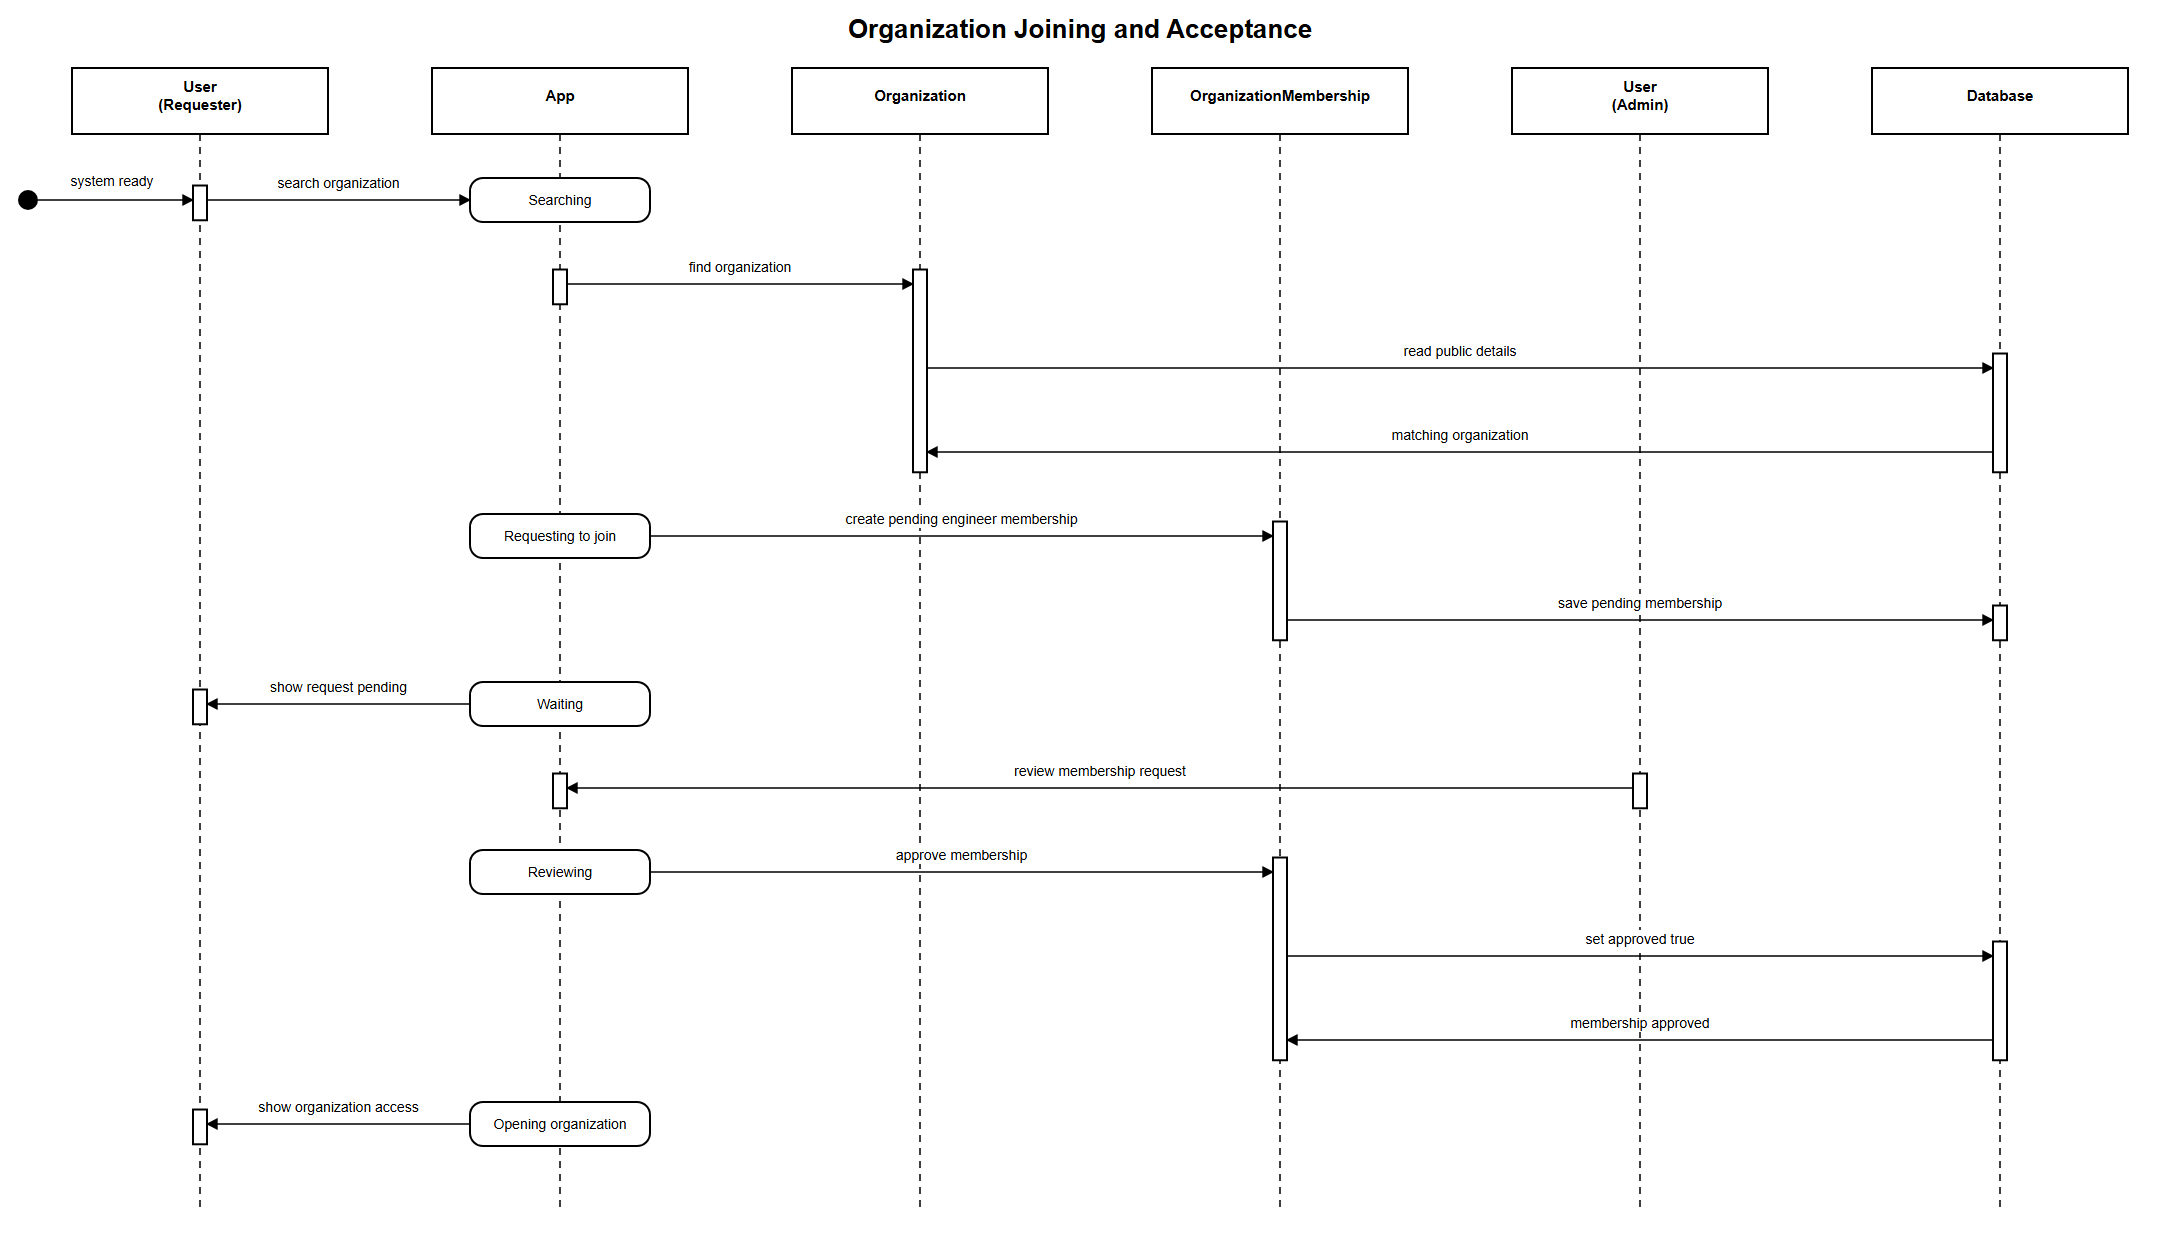
\includegraphics[width=0.92\textwidth]{Organization_Joining_and_Acceptance_Sequence_Diagram_1_.png}
\caption{Sequence diagram: Organisation Joining and Acceptance}\label{fig:seq_join}
\end{figure}

\begin{figure}[H]
\centering
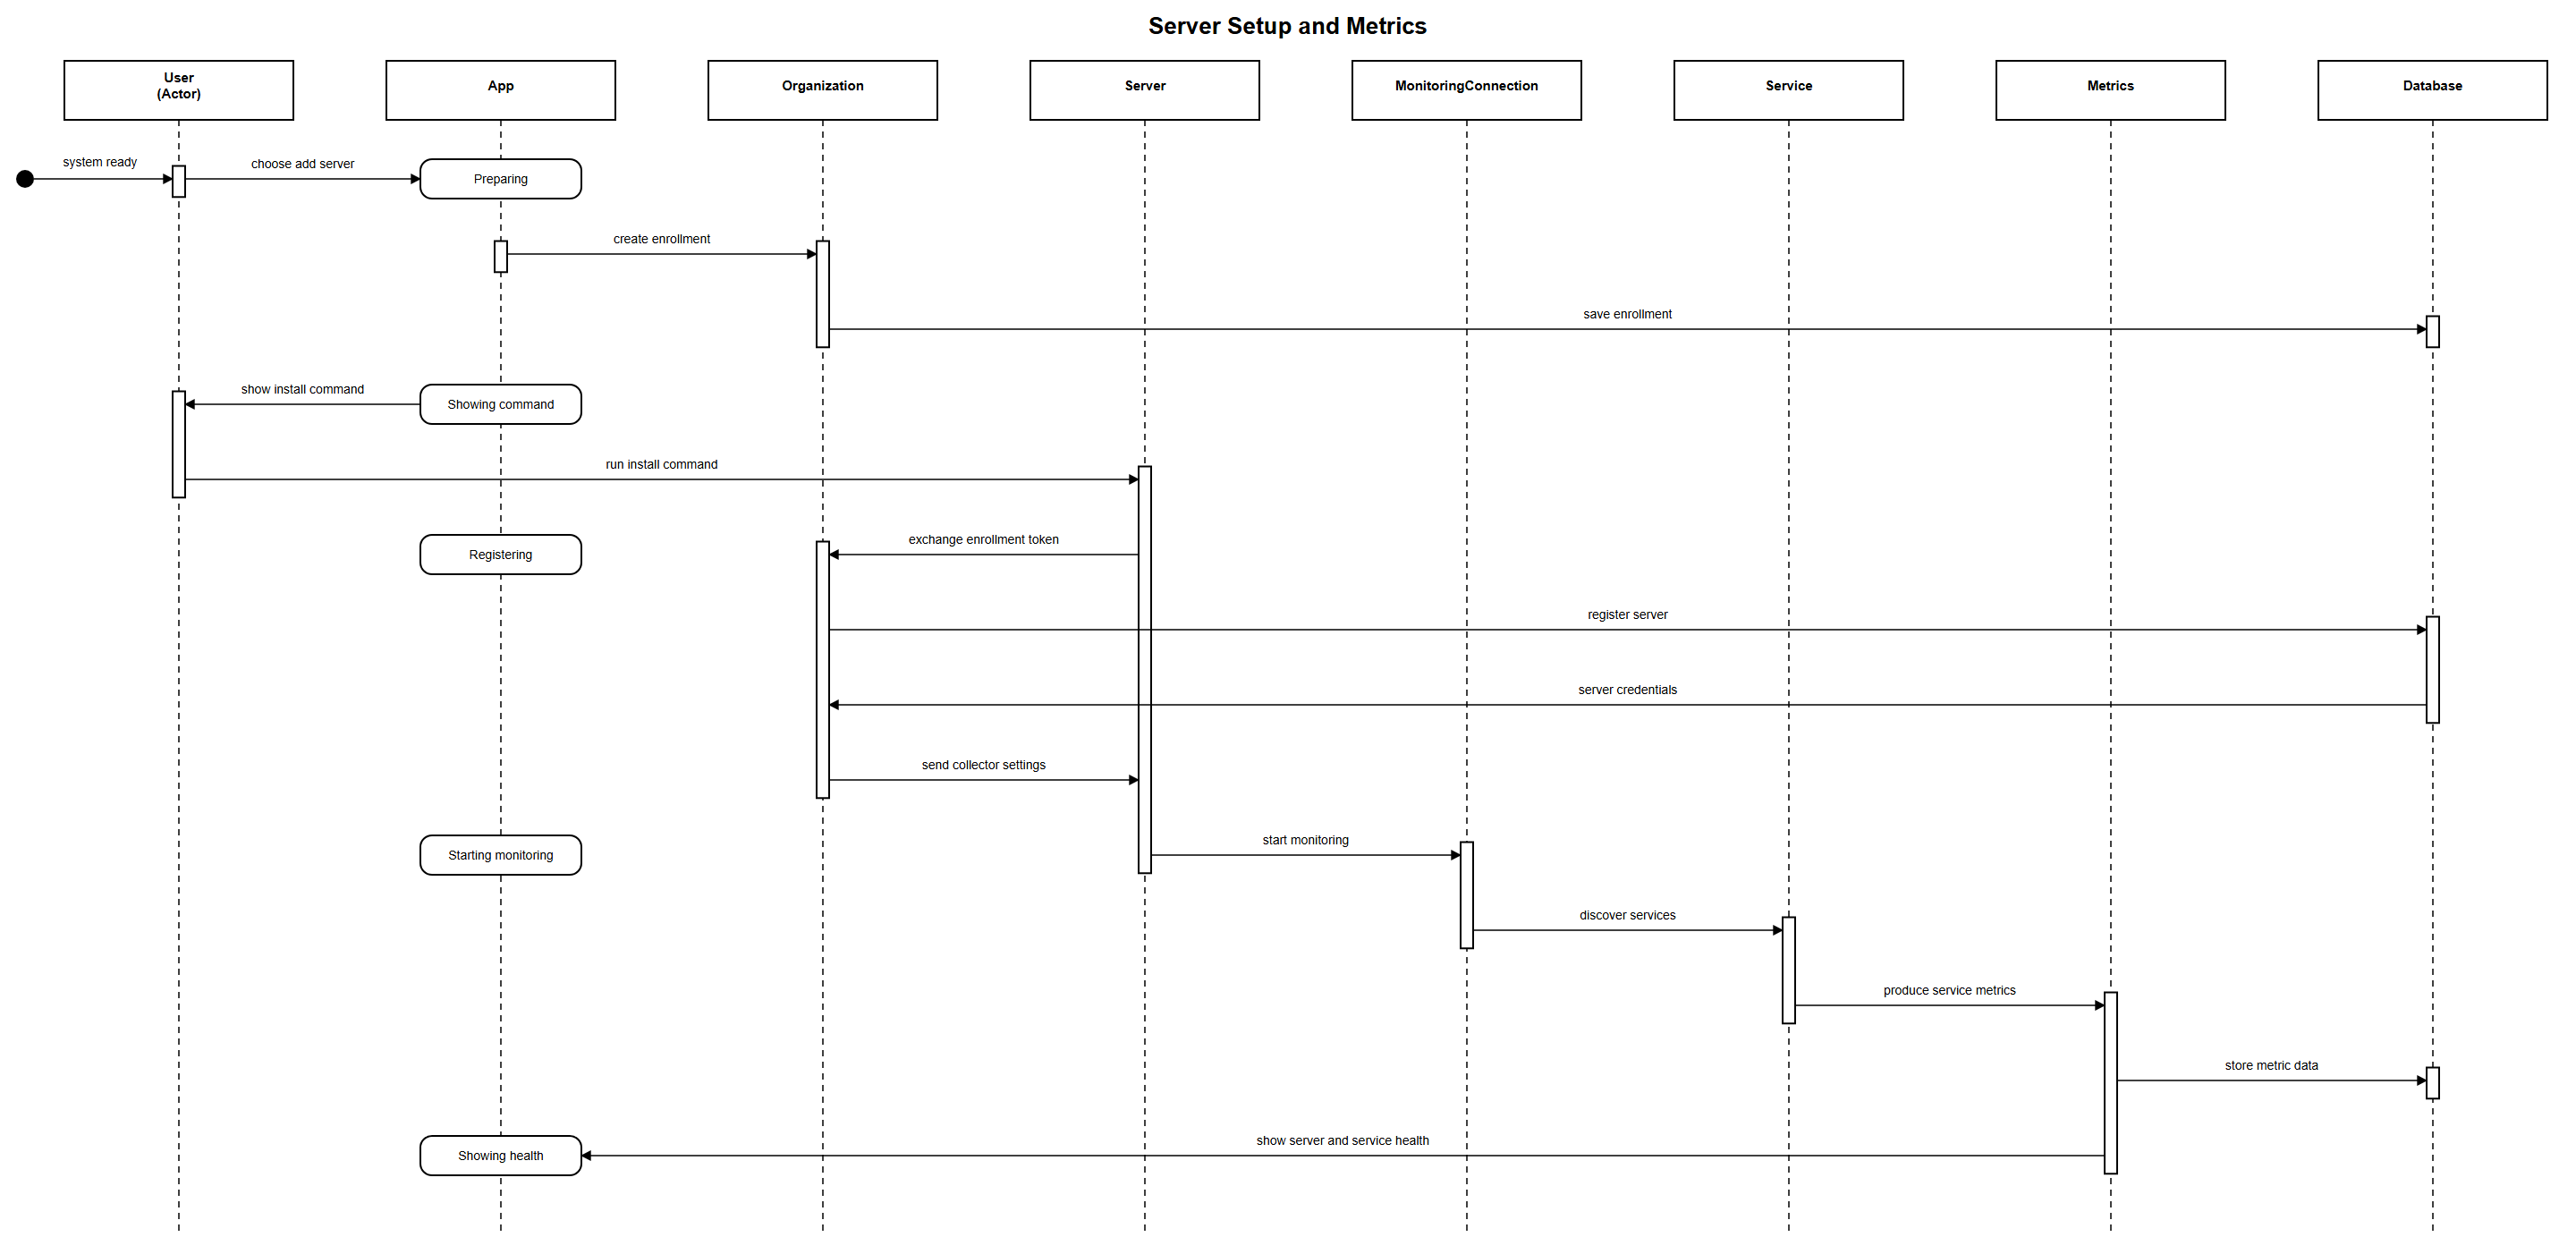
\includegraphics[width=0.92\textwidth]{Server_Setup_and_Metrics_Sequence_Diagram_1_.png}
\caption{Sequence diagram: Server Setup and Metric Collection}\label{fig:seq_server}
\end{figure}

\begin{figure}[H]
\centering
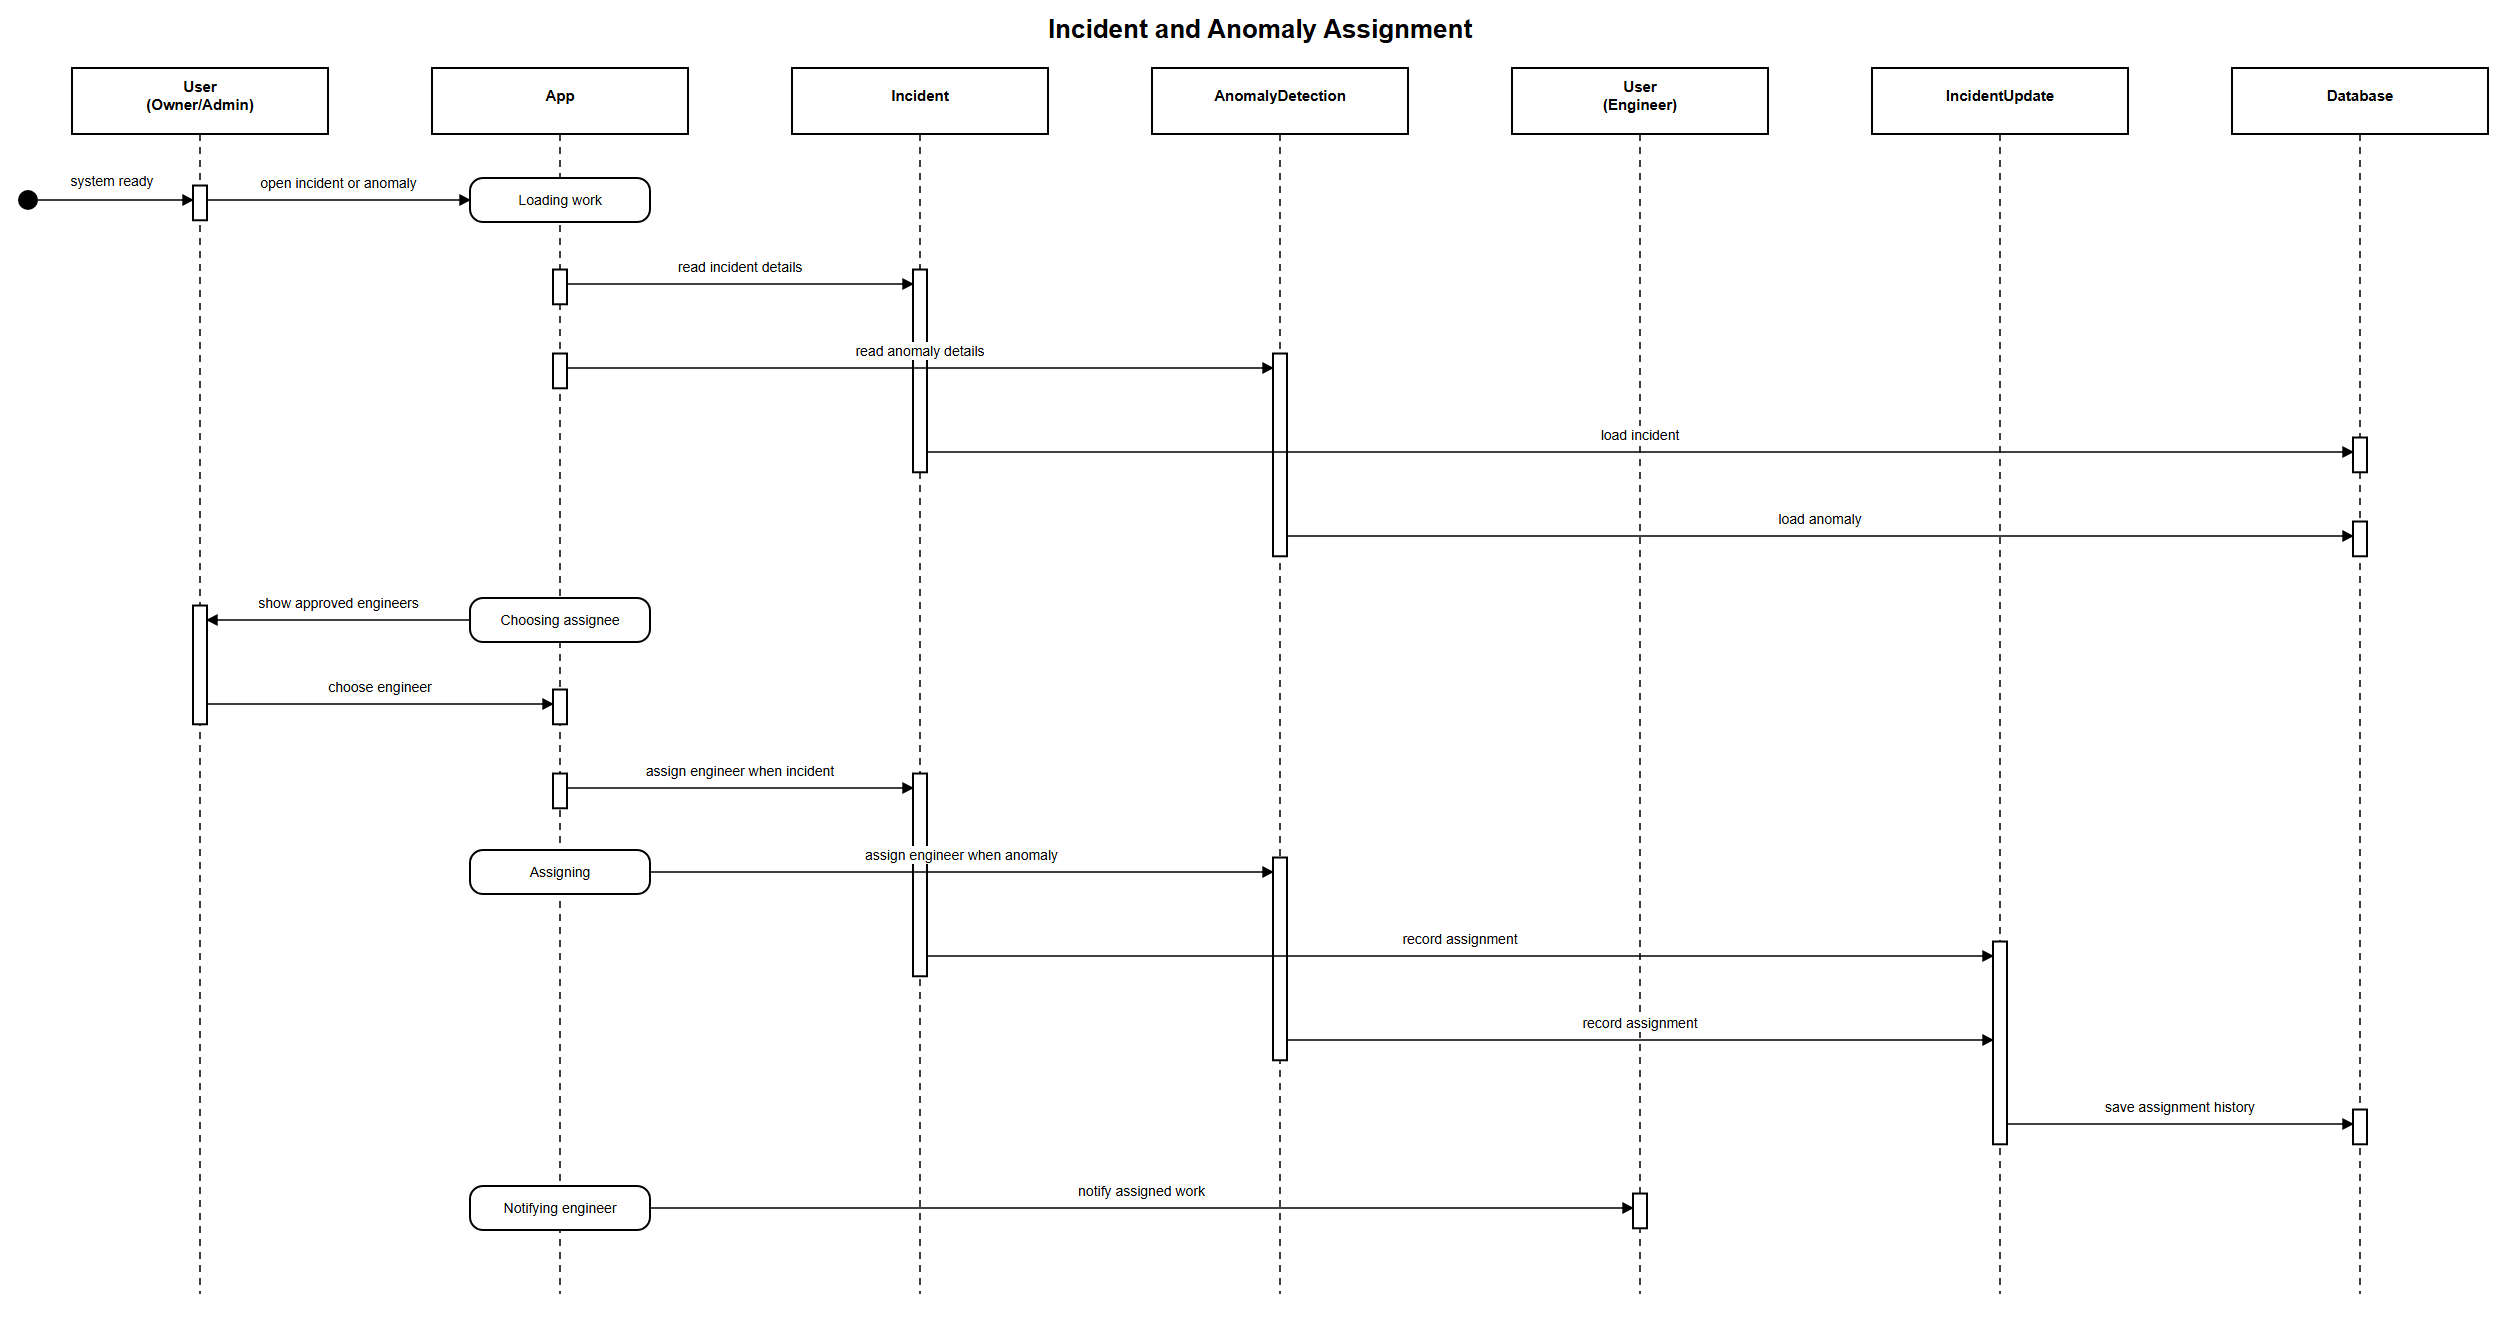
\includegraphics[width=0.92\textwidth]{Incident_and_Anomaly_Assignment_Sequence_Diagram_1_.png}
\caption{Sequence diagram: Incident and Anomaly Assignment}\label{fig:seq_incident}
\end{figure}

\begin{figure}[H]
\centering
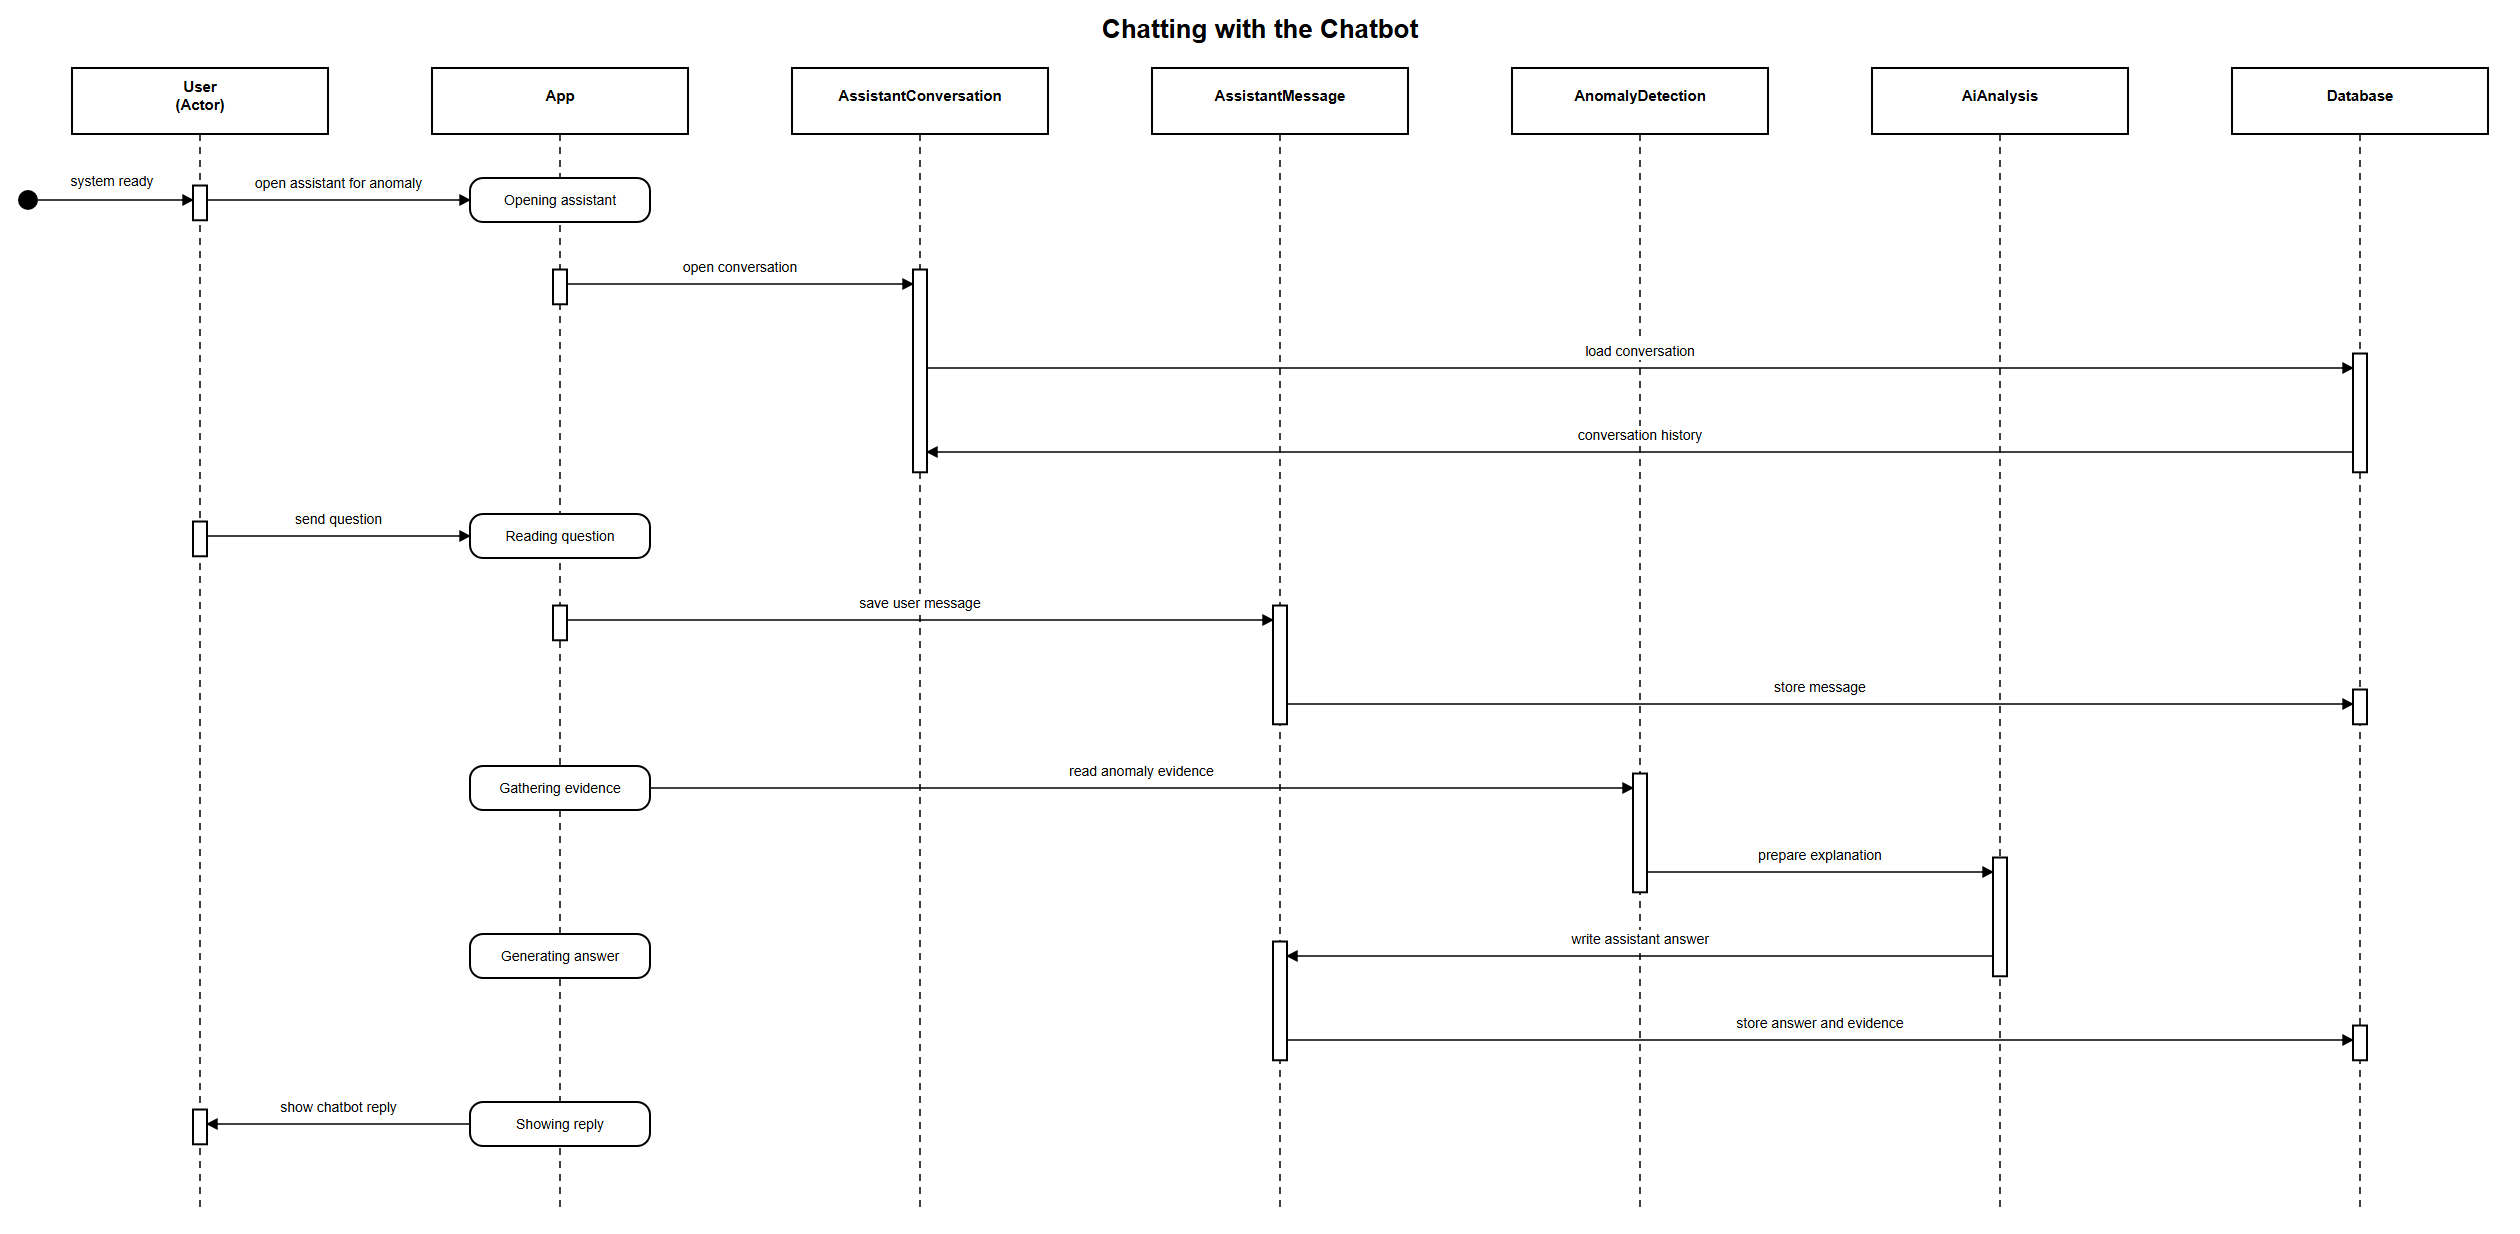
\includegraphics[width=0.92\textwidth]{Chatbot_Conversation_Sequence_Diagram_1_.png}
\caption{Sequence diagram: AI Chatbot (WebSocket) Conversation}\label{fig:seq_chatbot}
\end{figure}

\begin{figure}[H]
\centering
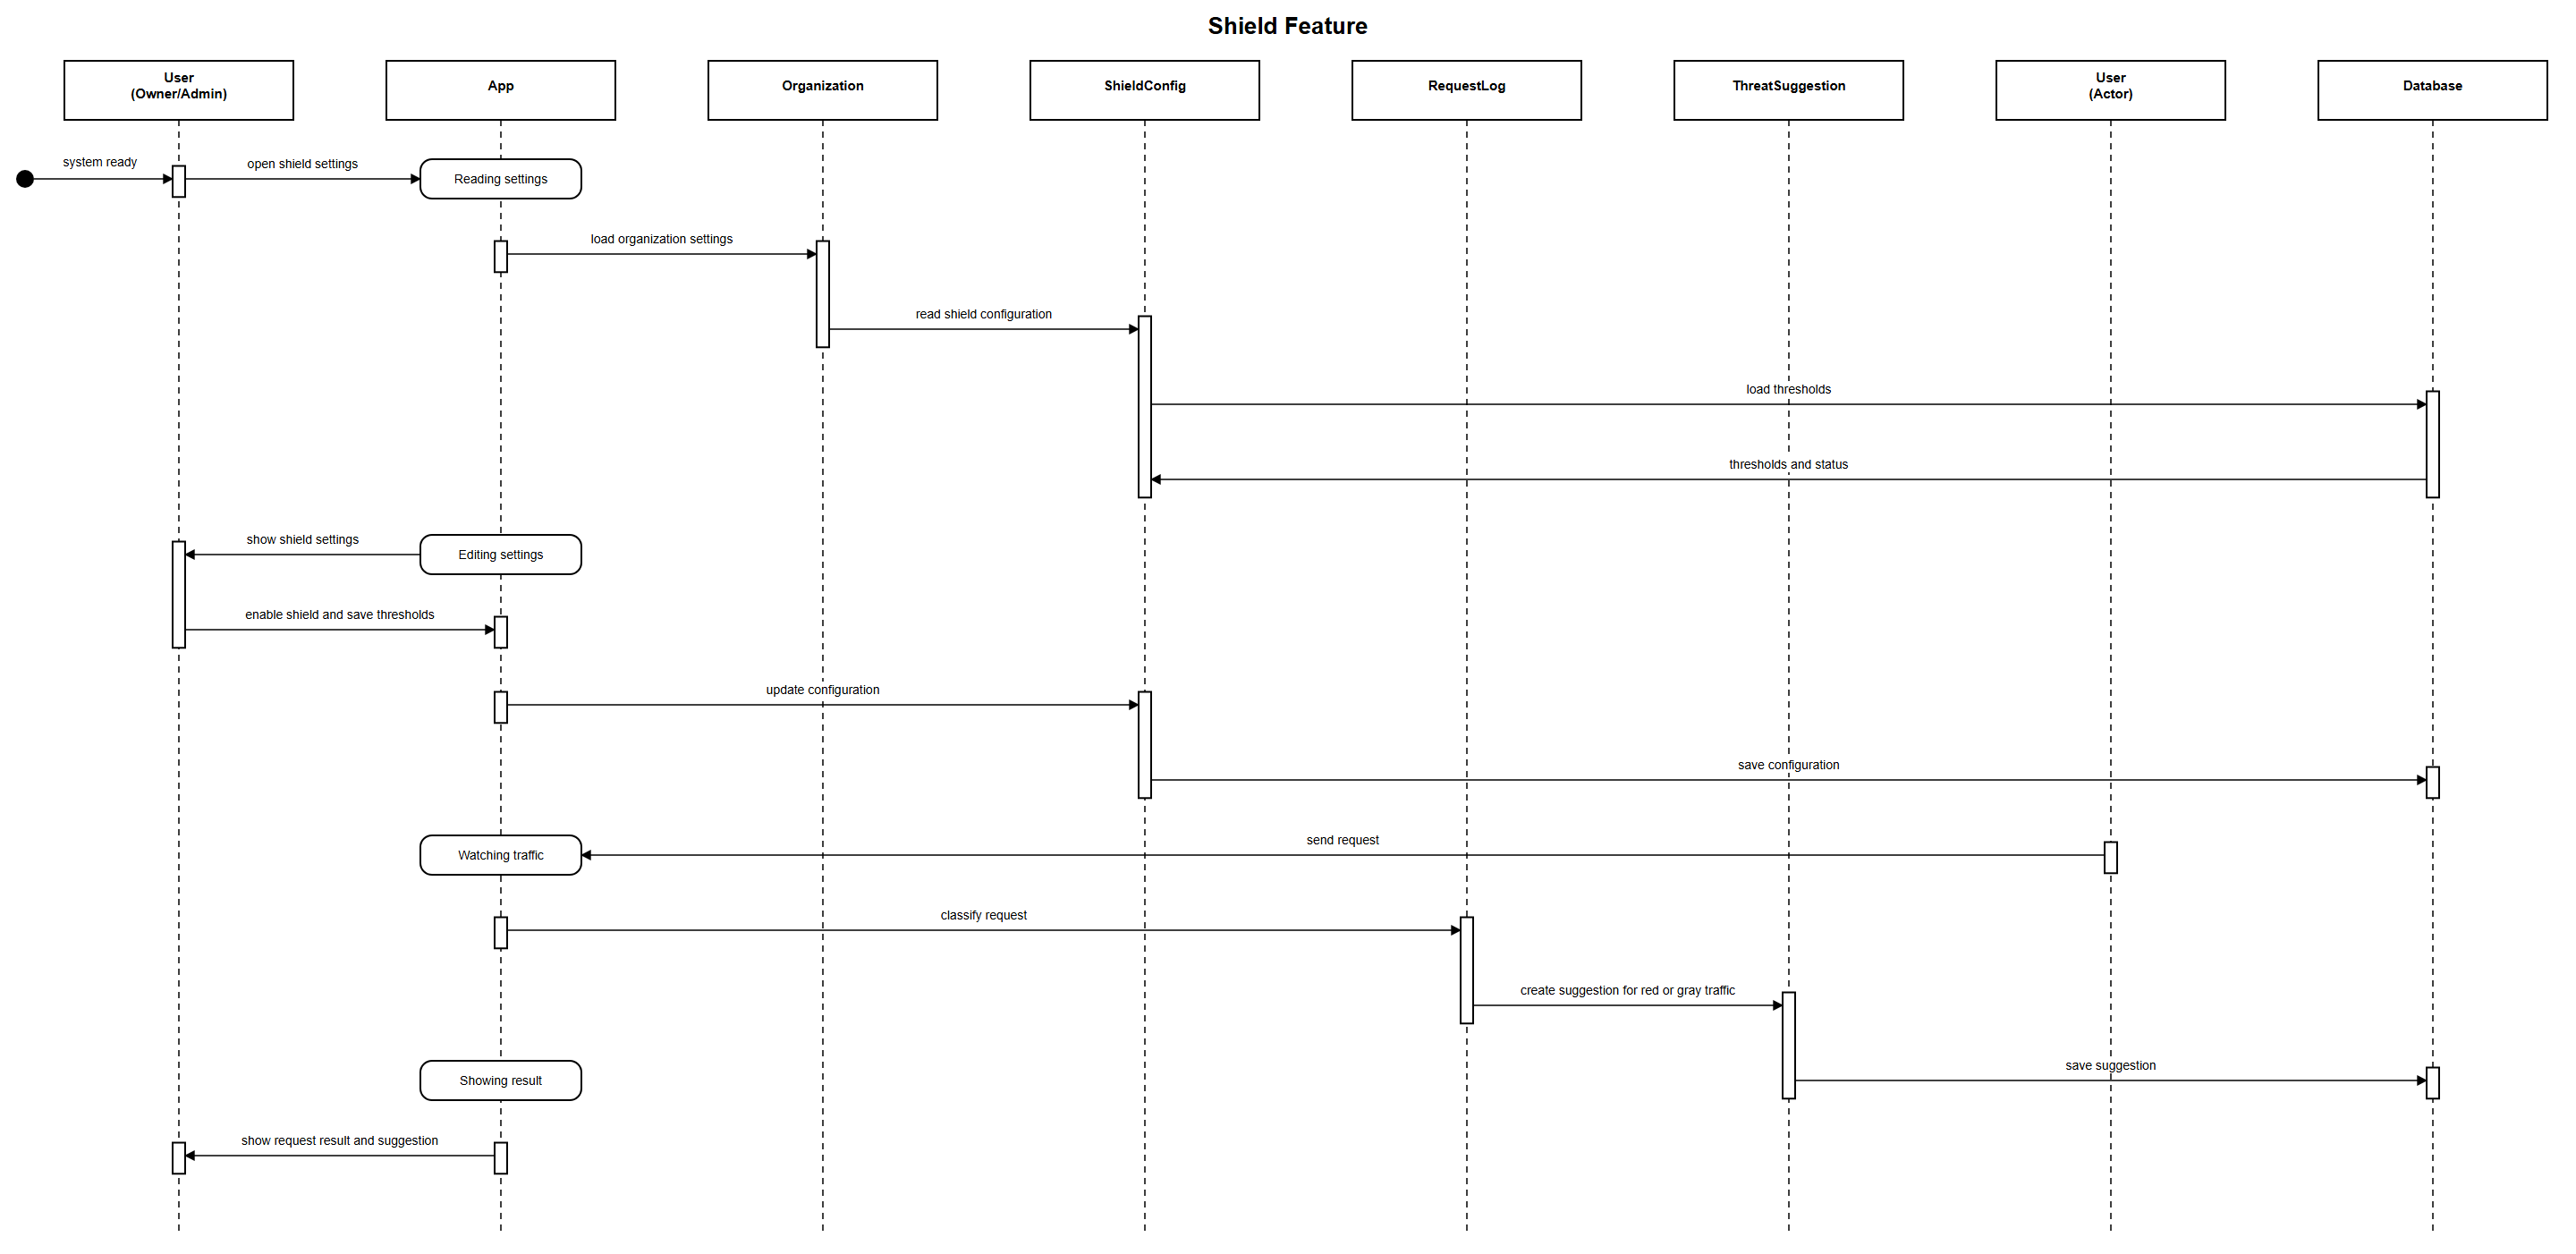
\includegraphics[width=0.92\textwidth]{Shield_Feature_Sequence_Diagram_1_.png}
\caption{Sequence diagram: Request Shield Classification and Threat Suggestion}\label{fig:seq_shield}
\end{figure}

\section{Safety and Security Requirements}

\subsection{Access Requirements}

Infra Monitor enforces a three-tier RBAC model implemented in
\texttt{accounts/models/organization\_membership.py}:

\begin{table}[H]
\centering
\caption{RBAC access control matrix}\label{tab:rbac}
\begin{tabularx}{\textwidth}{@{}l X c c c@{}}
\toprule
\textbf{Resource / Action} & \textbf{Description} & \textbf{Owner} & \textbf{Admin} & \textbf{Engineer}\\
\midrule
Register server & Create a new server in the org & \cmark & \cmark & \\
Approve membership & Approve join requests & \cmark & & \\
Assign service admin & Assign an Admin to a service & \cmark & & \\
Acknowledge / resolve alert & Change alert state & \cmark & \cmark & \\
Create / update incident & Full incident lifecycle & \cmark & \cmark & \\
Assign incident to engineer & Set \texttt{assigned\_to} field & \cmark & \cmark & \\
Resolve incident (assigned) & Update own assigned incident & \cmark & \cmark & \cmark \\
View dashboards / metrics & Read-only monitoring & \cmark & \cmark & \cmark \\
Use AI chatbot & Send messages, view conversations & \cmark & \cmark & \cmark \\
Request Shield admin & Verdict / suggestion actions & \cmark & \cmark & \\
\bottomrule
\end{tabularx}
\end{table}

Authentication is enforced via JWT Bearer tokens on all API endpoints through
\texttt{rest\_framework.authentication.JWTAuthentication}.  The
\texttt{common/api.py:get\_organization\_membership} helper validates that the
authenticated user has an approved membership in the requested organisation
before any domain view is executed.

\subsection{Integrity Requirements}

\begin{itemize}
  \item \textbf{Database constraints:} All models use UUID primary keys and
        Django's \texttt{UniqueConstraint} / \texttt{CheckConstraint} to enforce
        invariants at the database level (e.g., one OWNER per organisation,
        unique hostname per organisation, privileged memberships must be
        approved).
  \item \textbf{Model-level validation:} \texttt{clean()} methods on
        \texttt{Incident}, \texttt{AnomalyDetection}, \texttt{Alert}, and
        \texttt{ServiceAdminAssignment} validate cross-object references before
        save.
  \item \textbf{Atomic transactions:} Conversation creation uses
        \texttt{transaction.atomic()} with \texttt{get\_or\_create} to prevent
        duplicate rows under race conditions (\texttt{ai/views.py}).
  \item \textbf{Metric write integrity:} VictoriaMetrics vminsert enforces
        per-tenant data isolation; the backend proxies writes using the
        organisation's \texttt{VictoriaMetricsTenant.account\_id}.
\end{itemize}

\subsection{Privacy Requirements}

\begin{itemize}
  \item Passwords are stored as Django PBKDF2-SHA256 hashes; plaintext passwords
        are never logged or persisted.
  \item JWT access tokens are short-lived; refresh tokens are blacklisted on
        logout (\texttt{rest\_framework\_simplejwt.token\_blacklist}).
  \item WebSocket tickets are stored only as SHA-256 hashes
        (\texttt{ai/services.py:hash\_ticket}); the raw token is never persisted.
  \item Sanitized request log headers strip authentication cookies and tokens
        (\texttt{sanitize/models/request\_log.py} \texttt{headers\_digest} field docstring).
  \item Environment variables containing secrets (\texttt{SECRET\_KEY},
        \texttt{GEMINI\_API\_KEY}, \texttt{ML\_SERVICE\_TOKEN}) are loaded from
        \texttt{.env} files excluded from Git (\texttt{.gitignore}).
\end{itemize}

\section{AI-integration Requirements}

\begin{table}[H]
\centering
\caption{AI-integration requirements}\label{tab:airec}
\begin{tabularx}{\textwidth}{@{}l X l l@{}}
\toprule
\textbf{ID} & \textbf{Requirement} & \textbf{Must/Want} & \textbf{Metric}\\
\midrule
R-AI-01 & Isolation Forest shall flag anomalous service windows; precision $\geq$85\% &
  Must & Precision\\
R-AI-02 & Request Shield Random Forest shall achieve macro-F1 $\geq$0.90 on CICIDS2017 &
  Must & Macro-F1\\
R-AI-03 & Gemini chatbot shall stream first token within 5~s of user query &
  Want & Latency (p95)\\
R-AI-04 & Gemini response shall not execute commands or mutate system state
  (enforced by system prompt) & Must & Manual audit\\
R-AI-05 & Anomaly model shall be re-trainable when new labeled data exceeds
  10\% of original training set & Want & Retraining API\\
R-AI-06 & ML service health endpoint (\texttt{/health}) shall return 200 within 3~s &
  Must & Availability\\
R-AI-07 & Request Shield feature schema changes shall be versioned
  (\texttt{artifact\_format\_version}) & Must & Schema validation\\
R-AI-08 & Gemini escalation shall only be triggered for GRAY-zone requests
  to limit LLM API cost & Want & Cost constraint\\
\bottomrule
\end{tabularx}
\end{table}

